\documentclass[tg]{mdtufsm}

\usepackage{subcaption}
\usepackage{caption}
\captionsetup{
	justification=raggedright,
	figurewithout,labelsep=endash,
	singlelinecheck=false,
	compatibility=false
	}





\usepackage{chngcntr}
\counterwithout{figure}{chapter}
\counterwithout{table}{chapter}
\usepackage{ragged2e}
\usepackage{colortbl}
\usepackage{times}              % pacote para usar fonte Adobe Times
\usepackage{setspace}
\usepackage{array,multirow}
\usepackage{float} 
\usepackage[portuguese,titlenumbered,ruled]{algorithm2e} % algoritmos
\usepackage[T1]{fontenc}        % pacote para conj. de caracteres correto
\usepackage{fix-cm} %para funcionar corretamente o tamanho das fontes da capa
\usepackage{times, color, xcolor}       % pacote para usar fonte Adobe Times e cores
\usepackage[utf8]{inputenc}   % pacote para acentuação
\usepackage{graphicx}  % pacote para importar figuras
% % \usepackage{caption}
% \usepackage[]{subcaption}
\usepackage{amsmath,latexsym,amssymb} %Pacotes matemáticos
\usepackage[%hidelinks%, 
            bookmarksopen=true,linktocpage,colorlinks=true,
            linkcolor=black,citecolor=black,filecolor=magenta,urlcolor=blue,
            pdftitle={Título do Trabalho},
            pdfauthor={nome do autor},
            pdfsubject={Trabalho de Conclusão de Curso},
            pdfkeywords={modelo, latex, tcc, graduação}
            ]{hyperref} 

%Margens conforme MDT 2015
\usepackage[inner=30mm,outer=20mm,top=30mm,bottom=20mm]{geometry}
%algortmo definição
% \usepackage{algorithm}
% \usepackage{algorithmic}
% \floatname{algorithm}{Algoritmo}
% \renewcommand{\algorithmicfor}{\textbf{para}}
% \renewcommand{\algorithmicend}{\textbf{fim}}
% \renewcommand{\algorithmicendfor}{\textbf{fim de} \algorithmicfor}
% \renewcommand{\algorithmicdo}{\textbf{faça}}
%==============================================================================
% Se o pacote hyperref foi carregado a linha abaixo corrige um bug na hora
% de montar o sumário da lista de figuras e tabelas
% Se o pacote não foi carregado, comentar a linha %
%==============================================================================

%%=============================================================================
%% Trampa para corrigir o bug do hyperref que redefine o caption das figuras e das
%% tabelas, não colocando o nome ``Figura'' antes do número do mesmo na lista
%%=============================================================================

\makeatletter

\long\def\@caption#1[#2]#3{%
  \expandafter\ifx\csname if@capstart\expandafter\endcsname
                  \csname iftrue\endcsname
    \global\let\@currentHref\hc@currentHref
  \else
    \hyper@makecurrent{\@captype}%
  \fi
  \@ifundefined{NR@gettitle}{%
    \def\@currentlabelname{#2}%
  }{%
    \NR@gettitle{#2}%
  }%
  \par\addcontentsline{\csname ext@#1\endcsname}{#1}{%
    \protect\numberline{\csname fnum@#1\endcsname ~-- }{\ignorespaces #2}%
  }%
  \begingroup
    \@parboxrestore
    \if@minipage
      \@setminipage
    \fi
    \normalsize
    \expandafter\ifx\csname if@capstart\expandafter\endcsname
                    \csname iftrue\endcsname
      \global\@capstartfalse
      \@makecaption{\csname fnum@#1\endcsname}{\ignorespaces#3}%
    \else
      \@makecaption{\csname fnum@#1\endcsname}{%
        \ignorespaces
        \ifHy@nesting
          \expandafter\hyper@@anchor\expandafter{\@currentHref}{#3}%
        \else
          \Hy@raisedlink{%
            \expandafter\hyper@@anchor\expandafter{%
              \@currentHref
            }{\relax}%
          }%
          #3%
        \fi
      }%
    \fi
    \par
  \endgroup
}

\makeatother

%==============================================================================
% Identificação do trabalho
%==============================================================================
\title{Aprendizado por reforço para Navegação de Robôs Móveis}

\author{Costa de Jesus}{Junior}
%Descomentar se for uma "autora"
%\autoratrue

%% Lombada
\titulacao{Bacharel} %Tecn\'{o}logo ou Bacharel ou Licenciatura



%folha rosto
\course{Engenharia de Controle e Automação}
\initials{UFSM} 
\institute{Centro de Tecnologia}
\degree{Bacharel de Engenharia de Controle e Automação}

%CIP
\email{dranaju@gmail.com} %email do autor

% Número do TG (verificar na secretaria do curso)
% Para mestrado deixar sem opção dentro do {}
\trabalhoNumero{}

%Orientador
\advisoronepage[Prof.]{Dr.}{Fernado Tello Gamarra}{Daniel}
\advisor[Prof.]{Dr. (UFSM)}{Fernado Tello Gamarra}{Daniel}
%Se for uma ``orientadora'' descomentar a linha baixo
%\orientadoratrue

%Co orientador, comentar se não existir
%\coadvisor[Prof.]{Drª.}{Pereira}{Maria Regina}
%\coorientadoratrue %Se for uma ``Co-Orientadora''

%Avaliadores (Banca)
\committee[Me.]{Sobre nome}{Nome menbro banca}{UFSM}
\committee[Tecg.]{Sobre nome}{Nome menbro banca}{UFSM}

% a data deve ser a da defesa; 
% dia, mes e ano correntes
\date{03}{Julho}{2019} 

%Palavras chave
\keyword{Política de Gradiente Determinística Profunda}
\keyword{Ator-Crítica Suave}
\keyword{Aprendizado por Reforço Profundo} 
\keyword{Navegação de Robôs}

%keyword
\keywordAbstract{Deep Deterministic Policy Gradients}
\keywordAbstract{Soft Actor-Critic}
\keywordAbstract{Deep Reinforcement Learning}
\keywordAbstract{Robot’s Navigation}
%%=============================================================================
%% Início do documento
%%=============================================================================
\begin{document}
	
	

%%=============================================================================
%% Capa e folha de rosto
%%=============================================================================
\maketitle
%%=============================================================================
%% Catalogação (obrigatório para mestrado) e Folha de aprovação
%%=============================================================================
%Somente obrigatório para dissertação, para TG, remover as linhas	77	%
%Como a CIP vai ser impressa atrás da página de rosto, as margens inner e outer	
%devem ser invertidas.
\newgeometry{inner=20mm,outer=30mm,top=30mm,bottom=20mm} %%
\makeCIP{} 		
\restoregeometry

%Se for usar a catalogação gerada pelo gerador do site da biblioteca comentar as linhas
%\includeCIP{CIP.pdf}
	
%%=============================================================================
%folha de aprovação
%%=============================================================================
\makeapprove

%%=============================================================================
%% Dedicatória (opcional)
%%=============================================================================
% \chapter*{Dedicatória}


\vfill

\begin{center}
	
	{\sffamily\itshape Dedico este trabalho a ......}
	
\end{center}

\vfill

\newpage
%%=============================================================================
%% Agradecimentos (opcional)
%%=============================================================================
\chapter*{Agradecimentos}


\justifying{\textit{Agradeço .....}}



%%=============================================================================
%% Epígrafe (opcional)
%%=============================================================================
% \clearpage
\begin{flushright}
\mbox{}\vfill

{\sffamily\itshape
	\begin{quote}
		\begin{quote}
			\begin{quotation}
			``O valor de uma coisa depende da maneira como a abordamos mentalmente e não da coisa em si'' \\
			
			\begin{flushright}
			\textsc{(Jigoro Kano)}
		  	\end{flushright}
		  	
		\end{quotation}
		\end{quote}
	\end{quote}
 }




\end{flushright}

%%=============================================================================
%% Resumo
%%=============================================================================
\begin{abstract}
Esse trabalho apresenta um estudo da utilização das técnicas de aprendizado profundo usando a Política de Gradiente Determinística Profunda para a aplicação na navegação de robô móveis. 
Para realizar este trabalho foram utilizados os ambientes virtuais de simulação disponibilizados pela ROBOTIS no software de simulação Gazebo. 
Depois de feita a análise dos resultados, é possível concluir que o algoritmo de aprendizado por reforço profundo, com ações contínuas, é efetivo para a tomada de decisões de um veículo robótico. 
Porém, é preciso criar um sistema de recompensa para que o agente inteligente consiga assim cumprir seus objetivos.

\end{abstract}

%%=============================================================================
%% Abstract
%%=============================================================================
% resumo na outra língua
% como parametros devem ser passados o titulo, o nome do curso,
% as palavras-chave na outra língua, separadas por vírgulas, o mês em inglês
%o a sigla do dia em inglês: st, nd, th ...
\begin{englishabstract}
{Abstract title}
%%============ MANTER ESSA LINHA ============================================
\ %%============ MANTER ESSA LINHA ==========================================
%%============ MANTER ESSA LINHA ============================================
\ %%============ MANTER ESSA LINHA ==========================================
%%============ MANTER ESSA LINHA ============================================
\ %%============ MANTER ESSA LINHA e deixar uma em branco ===================

This paper presents a study of the use of deep learning techniques using the Deep Deterministic Policy Gradients for application on the navigation of mobile robots. 
The research studies for this case used the virtual simulation environments provided by ROBOTIS in the simulation’s software Gazebo.
After the analysis of the results, it is possible to conclude that the deep reinforcement learning’s algorithms, with continuous actions, are effective for decision-make of a robotic vehicle's decisions. 
However, it is necessary to create a reward’s systems for the intelligent agent can accomplish your objectives.

\end{englishabstract}

%% Lista de Ilustrações (opc)
%% Lista de Símbolos (opc)
%% Lista de Anexos e Apêndices (opc)

%%=============================================================================
%% Lista de figuras (comentar se não houver)
%%=============================================================================
\listoffigures
%%=============================================================================
%% Lista de tabelas (comentar se não houver)
%%=============================================================================
\listoftables

%%=============================================================================
%% Lista de Apêndices (comentar se não houver)
%%=============================================================================
%\listofappendix

%%=============================================================================
%% Lista de Anexos (comentar se não houver)
%%=============================================================================
%\listofannex

%%=============================================================================
%% Lista de abreviaturas e siglas
%%=============================================================================
 %o parametro deve ser a abreviatura mais longa

\begin{listofabbrv}{UbiComp}
	

	  \item [UFSM]      Universidade Federal de Santa Maria
	  \item [DNN]       Rede Neural Profunda
	  \item [FA]        Função de Ativação
	  \item [AI]        Inteligência Artificial
	  \item [GPU]       Unidade de Processamento Gráfica
	  \item [CPU]       Unidade Central de Processamento
	  \item [Deep-RL]   Aprendizado por Reforço Profundo
	  \item [TD]        Diferença Temporal
	  \item [DDPG]      Política de Gradiente Determinística Profunda
	  \item [SAC]       Ator-Crítica Suave
	  \item [ROS]       Sistema Operacional de Robôs
	  \item [IMU]       Unidade de Medição Inercial
	  \item [SBC]       Computador de Placa Única
	  \item [LDS]       Sensor de Distância \textit{Laser}
	  \item [OpenCV]    \textit{Open Source Computer Vision}

\end{listofabbrv}

%%=============================================================================
%% Lista de simbolos (opcional)
%%=============================================================================
%Simbolos devem aparecer conforme a ordem em que aparecem no texto
% o parametro deve ser o símbolo mais longo
%\begin{listofsymbols}{teste}
%  \item [$\varnothing$] vazio
 % \item [$\Gamma$]  Gama
%  \item [$\forall$] Para todo
%\end{listofsymbols}

%%=============================================================================
%% Sumário
%%=============================================================================
\tableofcontents











%%=============================================================================
%% Início da dissertação
%%=============================================================================
\setlength{\baselineskip}{1.5\baselineskip}


%%========================================================================
%Adiciona cada capitulo
\chapter{Introdução}

É observado atualmente um grande crescimento no campo da inteligência artificial (AI). 
Isso é devido a melhora do \textit{hardware} dos computadores atuais, que fazem com que os algoritmos mais recentes de AI sejam viáveis \cite{luo2005artificial}, principalmente com o aumento do poder computacional das unidades de processamento gráfico (GPU). 
As GPU’s tem como estrutura um processamento paralelo que torna mais eficientes os cálculos computacionais, em comparação a uma unidade central de processamento (CPU) \cite{asano2009performance}. 
A popularidade das GPU’s aconteceu também pela grande quantidade de dados gerados pela internet.

O Aprendizado por Reforço Profundo (Deep-RL) está começando a adquirir resultados interessantes em diferentes áreas, tais como: tarefas que envolvem o controle de sistemas discretos \cite{mnih2013playing}, sistemas contínuos \cite{lillicrap2015continuous}, e mais recentemente na robótica (\citeauthor{gu2017deep}, \citeyear{gu2017deep}; \citeauthor{mahmood2018benchmarking}, \citeyear{mahmood2018benchmarking}).
As primeiras aplicações de Deep-RL na robótica foram no uso de manipulação em ambientes totalmente observáveis e estáveis \cite{gu2016continuous}, mas tarefas em robótica móvel envolvem obstáculos que interagem com ambientes físicos e objetos, tornando assim o local de trabalho mais complexo.
Em ordem de resolver esse problema, métodos de Deep-RL normalmente tentam discretizar as ações para tornar o problema mais simples (\citeauthor{tai2016towards}, \citeyear{tai2016towards}; \citeauthor{zhu2017target}, \citeyear{zhu2017target}).
Em artigos recentes são exploradas técnicas para o controle contínuo de ações usado para navegação de robôs móveis com bons resultados (\citeauthor{tai2017virtual}, \citeyear{tai2017virtual}; \citeauthor{chen2017socially}, \citeyear{chen2017socially}).

\section{Descrição do Problema}
%estou aqui agora

O Deep-RL é definido como um campo da ciência que envolve treinos extensivos com redes neurais artificiais que usam de funções complexas, por exemplo, a dinâmica não-linear para mudar os dados brutos de um estado de alta dimensionalidade no qual pode ser entendido por um sistema robótico \cite{lecun2015deep}.
Usar o aprendizado de máquina para alcançar a tarefa de navegação autônoma em robôs móveis não é uma atividade simples como muitos pensam. 
O processo de percepção de um ambiente robótico e a interpretação das informações que ele adquire permitem compreender a condição de seu entorno, e assim fazer planos para mudar o estado e observar como suas ações impactam seu ambiente.
O desafio de navegar em um ambiente para os robôs móveis inclui problemas de movimento em locais com obstáculos variados, tornando assim o um ambiente complexo para um simples planejador de navegação \cite{shabbir2018survey}.

\section{Objetivos}

O desenvolvimento do projeto tem como objetivo utilizar as redes Deep-RL na tarefa de navegação de um robô móvel. Sua função é fazer com que um robô móvel, em um ambiente simulado e real, consiga chegar até um ponto alvo no mapa sem que a rede tenha um conhecimento prévio do ambiente. Espera-se que a agente inteligente chegue ao alvo sem colidir com nenhum obstáculo.

Concomitantemente, verificar o desempenho e resultados que tais redes podem oferecer na navegação de robôs móveís.

Objetivos específicos:
\begin{itemize}
\item Fazer a estrutura de redes Deep-RL capazes de descrever o problema da navegação, definindo-se uma entrada e saída desse sistema.
\item Criar um sistema de recompensas para que o robô móvel consiga completar a tarefa designada de chegar a um alvo determinado.
\item Aplicar a estrutura das redes e sistema de recompensas em ambientes simulados e reais.
\item Apresentar e medir os resultados obtidos nos ambientes testados das redes Deep-RL.
\end{itemize}



% \label{chap:Introducao}

% Está é a introdução do trabalho. Este modelo estar formatado conforme a MDT (Manual de Dissertação e Tese)da UFSM (Universidade Federal de Santa Maria) 20015. 

% Um bom livro de linguagens de programação é o \cite{Sebesta:2005}. 
% Conforme Sebesta \citeyearpar{Sebesta:2005}, uma boa linguagem de programação é Java \cite{Sun:2010}.

% Segundo Lee~\citeyearpar{Lee:2009}, a definição de contexto mais citada na bibliografia é a definição
% proposta por Abowd \textit{et al.}:

% \begin{quote}
%          Contexto é qualquer informação que pode ser utilizada 
%          para caracterizar a situação de uma entidade. Uma entidade é uma pessoa, lugar ou objeto que 
%          podem ser considerados relevantes para a interação entre um usuário e uma aplicação, 
%          incluindo o usuário e as suas próprias aplicações. \citep[tradução nossa]{Abowd:1999}
% \end{quote}

% Outras referências: \cite{Alex:2010}, \cite{Weiser:1991} e \cite{norell:thesis}.

% \section{Objetivos}
% O objetivo deste trabalho é .....

% \section{Tabela}
% Um exemplo de tabela é a \ref{tabrecursosdisp1}:



% \begin{table}[!ht]
% 	\caption{Comparação entre recursos disponíveis}
% 	\begin{center}
% 		\begin{tabular}{ll|ll}
% 			\hline
% 			\multicolumn{2}{c}{Cacti}       & \multicolumn{2}{|c}{Zabbix}                   \\ \hline
% 			& CPU usage                     & CPU jumps                                  &  \\ \hline
% 			& CPU utilization               & CPU load                                   &  \\ \hline
% 			& Load usage                    & CPU utilization                            &  \\ \hline
% 			& Load averge                   & Disk space usage                           &  \\ \hline
% 			& Logged in users               & Memory usage                               &  \\ \hline
% 			& Memory usage                  & Network traffic on eth0                    &  \\ \hline
% 			& Ping Latency                  & Network traffic on eth2                    &  \\ \hline
% 			& Traffic (bits/sec)            & Swap usage                                 &  \\ \hline
% 			&                               & Value cache effectiveness                  &  \\ \hline
% 			&                               & Zabbix cache usage, \% free                &  \\ \hline
% 			&                               & Zabbix data gathering process busy         &  \\ \hline
% 			&                               & Zabbix internal process busy               &  \\ \hline
% 			&                               & Zabbix server performance                  &  \\ \hline
% 		\end{tabular}
% 	\end{center}
% 	\small{Fonte:Adaptado de \cite{dos2016comparativo}.}
% 	\label{tabrecursosdisp1}
% \end{table}
\chapter{Revisão de Literatura}

Neste capítulo são descritos os trabalhos que serviram de inspiração para o projeto. 
Do mesmo modo, é feito a revisão teórica das técnicas que serão aplicadas para a resolução do problema que o projeto propõe resolver.

\section{Trabalhos Relacionados}

O Deep-RL já foi aplicado anteriormente em tarefas que envolvem robótica, entre essas aplicações podem ser referenciado os trabalhos de (\citeauthor{kober2013reinforcement}, \citeyear{kober2013reinforcement}; \citeauthor{stone2005reinforcement}, \citeyear{stone2005reinforcement}).
Mnih \citeyearpar{mnih2013playing} utilizou de rede neural convolucional para estimar uma função de valor para recompensas futuras no jogos eletrônicos do Atari, essa estratégia foi chamada de \textit{Deep Q-learning}.
A \textit{Deep Q-learning} pode ser apenas usada em uma tarefa que tenha ações discretas. Para estendê-lo para o controle contínuo, Lillicrap \citeyearpar{lillicrap2015continuous} propôs uma política de gradiente determinística profunda.
Essa tornou a base para as aplicações de Deep-RL na navegação de robôs móveis, assim como, na criação de novas técnicas como actor-crítica suave \cite{haarnoja2018soft}.

Tai \citeyearpar{tai2017virtual} criou um planejador de movimento sem mapeamento para um robô móvel pegando 10 leituras de um sensor \textit{laser} e a posição de um alvo em relação ao robô como entrada, e os comandos de direção contínuos como saída da rede, mas sendo primeiramente proposto como comandos de direção discretos \cite{tai2016towards}. Foi mostrado que, com métodos assíncronos de Deep-RL, um planejador de movimento sem mapeamento pode ser treinado e completar a tarefa de chegar a um algo determinado.

Zhu \citeyearpar{zhu2017target} propôs um outro modelo para aplicar Deep-RL para a tarefa de dirigir um robô móvel. O modelo criado toma a obervação atual de estado e a imagem do alvo como entrada e gera uma ação em um ambiente de três como saída.

Uma atividade que pode ser muito desafiante na robótica é navegar um veículo com segurança e eficiência em ambientes com muitos pedestres. Chen \citeyearpar{chen2017socially} elaborou um modelo Deep-RL que pode quantificar o que fazer e não fazer no mecanismo de navegação humana.
Este trabalho desenvolveu uma politica de navegação eficiente de tempo que respeita normas sociais comuns. Criando assim um método capaz de controlar um robô móvel que se move na velocidade de caminhada humana em um ambiente com muitos pedestres.,


\section{Aprendizado de Máquina}

O aprendizado de máquina é um ramo da inteligência artificial baseada na ideia que sistemas podem aprender através de dados, identificar padrões e fazer decisões com a intervenção mínima de humanos \cite{mitchell1990machine}. Expandindo seus estudos para algoritmos e modelos estatísticos que sistemas computacionais usam para melhorar seu desempenho em tarefas específicas.

É possível classificar o aprendizado de máquina em 3 grandes categorias:
\begin{itemize}
    \item Aprendizado supervisionado: este aprendizado consiste em um sistema que possui variáveis de entrada e variáveis de saída. As variáveis de entradas são referentes a uma variável de saída determinada e o aprendizado é chamado supervisionado, pois a variável de saída, durante o treino, já é conhecida pelo algoritmo. A função desse sistema é fazer com que o algoritmo possa maximizar as predições de saída para uma resposta correta que é conhecida previamente pela rede.
    \item Aprendizado não-supervisionado: consiste em um sistema que apenas possui variáveis de entrada sem uma saída correspondente. O objetivo desse tipo de aprendizado é modelar estruturas que possam dizer mais sobre o conjunto dos dados que estão sendo estudados.
    \item Aprendizado por reforço: neste tipo de aprendizado o agente inteligente interage com um ambiente dinâmico, para desempenhar um determinado objetivo. É fornecido, ao agente, o \textit{feedback} quanto a premiações e punições, na medida em que é explorado o espaço de solução.
\end{itemize}

\subsection{Aprendizagem profunda}

A aprendizagem profunda é uma subcategoria do aprendizado de máquinas \cite{lecun2015deep}.
Semelhante ao aprendizado de máquina, o aprendizado profundo também possui aprendizado supervisionado, não-supervisionado e de reforço.
O algoritmo de aprendizagem profunda depende de redes neurais profundas. 
Redes neurais profundas podem automaticamente achar representações compactas de baixa dimensionalidade de dados com alta dimensionalidade (e.g., imagens, texto e audio) \cite{arulkumaran2017brief}.
Essas redes neurais foram baseadas no funcionamento dos neurônios do cérebro humano. 
Ou seja, o aprendizado profundo vem dá criação de redes neurais que possuem neurônios que se comunicam entre si e conseguem passar informação. 

Uma Rede Neural Profunda (DNN) consiste de múltiplas camadas de unidades de processamento não-linear (camada escondida). Ela executa a extração e transformação de características. Na Figura \ref{fig:NN} é mostrada uma DNN que consiste que três camadas: camada de entrada, camadas escondidas e camada de saída. Na camada de entrada, os neurônios são generalizados a partir de recursos que passam por sensores que percebem o ambiente. As camadas escondidas podem incluir uma ou mais camadas. A camada de saída contem a saída desejada, por exemplo, a distribuição de todas as ações possíveis.
Cada camada sucessiva da DNN usa a saída da camada anterior como entrada.
Todos os neurônios das camadas são totalmente ativados através de conexões ponderadas.

\begin{figure}[H]
\caption{Rede Neural Simples e Profunda}
\centerline{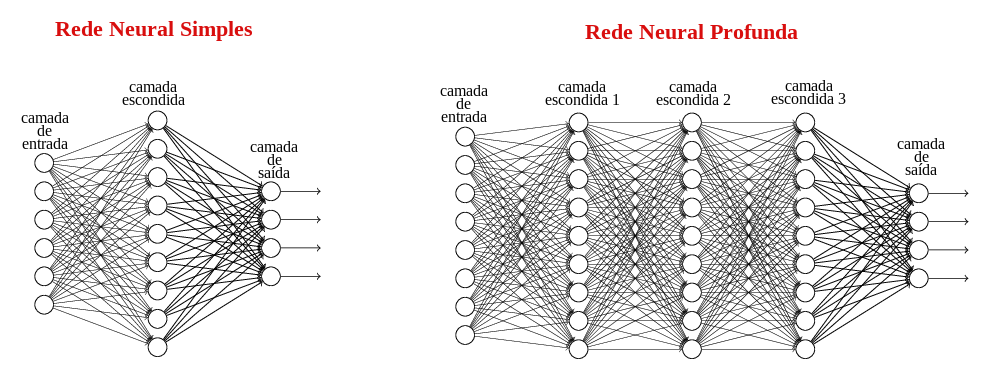
\includegraphics[width=\columnwidth]{imagens/neural_network.png}}
\small{Fonte: http://neuralnetworksanddeeplearning.com/chap5.html}
\label{fig:NN}
\end{figure}

Todas as DNN são funções matemáticas. 
Então, para calcular a função de uma camada é usado a definição abaixo:
\begin{equation}
    a^{(c)} = W a^{(c-1)} + b
    \label{eq:camada}
\end{equation}

Sendo os neurônios da camada atual $a^{(c)}$ e da camada anterior $a^{(c-1)}$, os pesos de todas as conexões entre as duas camadas $W$ e um número pré-determinado de bias $b$.

Contudo, em aplicações do mundo real, funções lineares não conseguem descrever todos os sistemas, quase sempre, funções não-lineares são usadas. Para fazer isso é preciso aplicar uma função não-linear, conhecida como função de ativação (FA), a Equação \ref{eq:camada}, que ficaria definida como:
\begin{equation}
    a^{(c)} = FA\left\{W a^{(c-1)} + b\right\}
\end{equation}

Então, para resolver sistemas não-lineares diferentes funções de ativação podem ser usadas ou pode ser criada a própria função de ativação que se ajusta ao problema. Existem diversas FA's pré-definidas, tais como: `linear', `ReLU', `tanh', `sigmoid', etc.
Na Figura \ref{fig:FA} é mostrada a respostas para as FA's mais conhecidas.

\begin{figure}[H]
\caption{Exemplos de resposta de funções de ativação}
\centerline{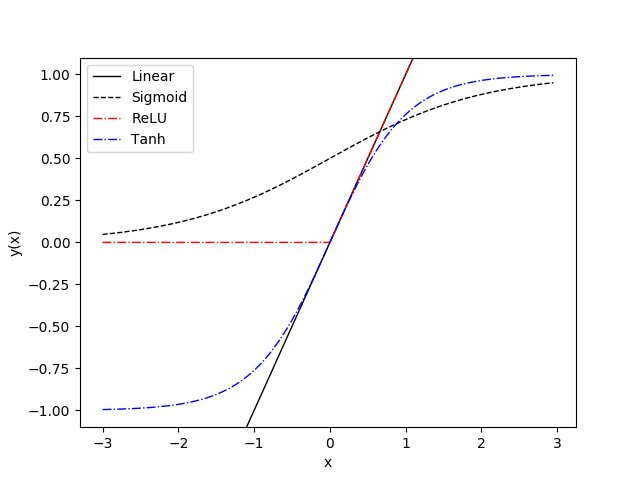
\includegraphics[width=\columnwidth]{imagens/function_activation.png}}
\small{Fonte: Autor}
\label{fig:FA}
\end{figure}

Depois do fluxo de computação avançar da entrada para a saída, na camada de saída e cada camada escondida, é possível calcular o erro derivativo para propagar os gradientes em direção a camada de entrada, sendo assim os pesos podem ser atualizados para otimizar a função de perda \cite{li2017deep}. Isto é o foco da parte de aprendizagem, para achar os pesos e bias certos.

% Geralmente utiliza-se de redes neurais e de muitos dados para o seu treinamento. 
% Essas redes neurais foram baseadas no funcionamento dos neurônios do cérebro humano. Ou seja, o aprendizado profundo vem dá criação de redes neurais que possuem neurônios que se comunicam entre si e conseguem passar informação. 
% E enquanto, programas tradicionais constroem análises com dados de uma forma linear, o aprendizado profundo constrói funções hierárquicas para o processamento de dados de uma forma não linear.

% Uma rede neural, na sua forma mais simples, é composta de múltiplas camadas de nós interconectados, como é mostrado na Figura 3. 
% As conexões da rede são similares as conexões dos neurônios do cérebro humano. 
% A conexão entre as camadas possuem um nó e a este nó está associado a um peso. 
% A rede neural é treinada pelo uso de grandes conjuntos de dados rotulados que aprendem características diretamente dos dados sem a necessidade da intervenção manual.

% figura

% A rede neural pode apresentar um maior número de camadas escondidas assim podendo-se classificar como uma rede “profunda”.
% Em uma rede neural com múltiplas camadas escondidas, o número de parâmetros cresce exponencialmente, podendo assim ter uma melhor eficiência para a resolução de problemas que uma rede neural de apenas uma única camada escondida.

% Muitos dos modelos modernos de aprendizado profundo são baseados em uma rede neural artificial. Cada nível da rede aprende a transformar as informações de entrada em algo  mais abstrato. 
% Como regra, quanto mais profunda é o modelo, mais a rede tem potencial de obter um melhor desempenho que os modelos mais superficiais. 
% O problema é que quanto mais profunda é a rede, mais dados são necessários para evitar o sobreajuste, sem falar, do aumento do tempo para obter uma resposta de saída.
% No caso de uma rede que vá cuidar de um robô, em constante movimento, é preciso ter uma resposta mais rápida. Logo, uma rede superficial é melhor para esse tipo de aplicação.

\subsection{Aprendizado por Reforço}

O aprendizado por reforço é uma área de aprendizado de máquina que lida com tomada de decisão sequencial.
Um aspecto chave do aprendizado por reforço é que um agente aprenda uma bom comportamento \cite{franccois2018introduction}.
Isso significa que ele modifica ou adquiri novos comportamentos e habilidades incrementalmente.
Um outro importante aspecto do aprendizado por reforço é que ele usa de experiência de tentativa e erro.
Ademais, o agente do aprendizado por reforço não precisa de completo conhecimento ou controle do ambiente; ele apenas precisa ser capaz de interagir com o ambiente e coletar informações.
Um agente realiza certas ações em um ambiente e um interpretador dá uma recompensa para o novo estado do agente, tendo assim um ciclo entre as ações e interpretações feitas no ambiente, como é mostrado na Figura \ref{fig:ciclo_rl}.

\begin{figure}[H]
\caption{Interação do agente no ambiente em aprendizado por reforço}
\centerline{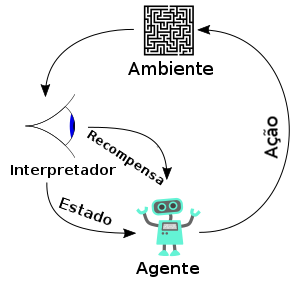
\includegraphics[width=10cm]{imagens/ciclo_rl_agente.png}}
\small{Fonte: Super Data Science}
\label{fig:ciclo_rl}
\end{figure}

O aprendizado por reforço possui dois tipos de configuração, o \textit{offline} e \textit{online} como é chamado na literatura \cite{sutton1998introduction}. Em uma configuração \textit{offline}, a experiência adquirida \textit{a priori} e então é usada para o aprendizado. Isso é um contraste com a configuração \textit{online} onde os dados tornam disponíveis em uma ordem sequencial e são usados para progressivamente atualizar o comportamento do agente.

\subsubsection{Processo de decisão de Markov}

A forma básica de modelar o aprendizado por reforço é seguindo um processo de Markov. O processo de Markov é definido como a probabilidade do estado futuro depender apenas do estado atual \cite{bellman1957markovian}. Sem depender de nenhuma das ações e estados anteriores. Isso quer dizer:
\begin{equation}
P(s_{t+1} \mid {s_0,a_0,s_1,a_1 , ... ,s_t,a_t}) = P( s_{t+1} \mid {s_t,a_t} )
\label{eq:eq1}
\end{equation}

Para um agente que está em um estado e realiza uma certa ação em um ambiente, acontecerá com que o depois dessa ação o agente se encontre em um novo estado em relação ao estado anterior, e então uma determinada recompensa é dada pela ação tomada. A função de recompensa define a meta que o agente do aprendizado por reforço deve atingir. O objetivo desse agente é maximizar a recompensa que ele recebe ao longo do tempo.

Então com a abordagem do agente que utiliza o conceito do processo de Markov, para cada tempo t, são usados os seguintes passos:
\begin{enumerate}
    \item O agente observa o estado atual $s_t$.
    \item O agente faz a ação $a_t$.
    \item O agente recebe a recompensa $r_t = R(s_t, a_t)$.
    \item O agente entra no próximo estado $s_{t+1}$.
\end{enumerate}

Sabendo que na abordagem do processo de Markov é necessário utilizar a equação de Bellman, que especifica qual é a melhor ação que um agente deve tomar em um certo estado \cite{bellman2015applied}. Isto é, a equação de Bellman consegue prever a recompensa gerada de um estado para outro, enquanto, que a função de recompensa só pensa no que é bom em um sentido imediato. A Equação de Bellman é definida como:
\begin{equation}
    V( s_{t} ) =  \underset{a_t}{max}(R(s_t,a_{t}) + \gamma V(s_{t+1}))
    \label{eq:eq2}
\end{equation}

Essa fórmula nos diz qual é o maior valor do estado depois de tomada uma ação.
`$V$' é definido como a “valor” do estado no ambiente.
O valor $\gamma$ (gama) é para admitir um valor de desconto para cada ação tomada. Com a Equação \ref{eq:eq1} e a Equação \ref{eq:eq2} definidas, considerando todas as ações possíveis que um agente pode tomar e a probabilidade de cada ação, é possível ter a equação do processo de decisão de Markov, que é definida como:
\begin{equation}
    V( s_{t} ) = \underset{a_t}{max}( R(s_t,a_{t}) + \gamma \sum_{s_{t+1}} P( s_{t+1} \mid {s_t,a_t} ) V(s_{t+1}) )
\end{equation}

Antes do processo de decisão de Markov, o que acontecia é que todas ações eram tomadas em um ambiente determinístico. Mas com a inserção de incerteza nas ações é possível modelar um ambiente de predição melhor para um lugar mais abstrato e estocástico.

\subsection{Q-Learning}

A diferença de um agente que toma suas decisões pelo processo de decisão de Markov e \textit{Q-Learning} é que em uma abordagem do Markoviana o agente olha a qualidade dos estados futuros baseados no estado atual, enquanto que em \textit{Q-Learning} o agente olha para a qualidade de cada ação sabendo o estado atual \cite{watkins1992q}. 
‘Q’ é definido como a “qualidade” da ação de um agente em um estado e a função retornada é a recompensa dessa ação. É possível derivar a fórmula para o \textit{Q-Learning} através da abordagem de Markov, gerando a seguinte equação:
\begin{equation}
    Q( s_{t}, a_t ) = R(s_t,a_{t}) + \gamma \sum_{s_{t+1}} P( s_{t+1} \mid {s_t,a_t} ) \underset{a_{t+1}}{max} (Q(s_{t+1}, a_{t+1}))
    \label{eq:eq4}
\end{equation}

Mesmo depois de achar o valor de `$Q$' causado por uma ação, é preciso lembrar que o agente precisa percorrer esse ambiente provavelmente mais de uma vez. 
Então se for mantida a ideia da equação \ref{eq:eq4}, nunca será possível que um agente inteligente possa aprender, pois essa fórmula permite apenas atualizar os valores de `$Q$' para uma certa ação que aconteceu no tempo atual, sem levar em conta se a ação foi boa ou ruim.
Para corrigir isso é preciso considerar uma diferença temporal e uma taxa de aprendizado ($\alpha$) para que assim seja possível que o algoritmo melhore seu desempenho com o tempo, mesmo que faça ações que não beneficiem o agente. 
Ou seja, é possível definir as seguintes equações:

\begin{enumerate}
    \item A equação da diferença temporal entre os valores de Q:
    \begin{gather}
        TD_t = \Delta Q( s_t,a_t )\\
        TD_t = R(s_t,a_{t}) + \gamma \sum_{s_{t+1}} P( s_{t+1} \mid {s_t,a_t} ) \underset{a_{t+1}}{max} (Q(s_{t+1}, a_{t+1}) - Q_{t-1}(s_{t}, a_{t}))
    \end{gather}
    
    \item A equação que atualizar o valor de Q para cada ação que passou por aquele estado:
    \begin{equation}
        Q_t ( s_t,a_t ) = Q_{ t-1 }( s_t,a_t )+ \alpha TD_t( s_t,a_t )
        \label{eq:q_function}
    \end{equation}
\end{enumerate}

Com a equação \ref{eq:q_function} definida é possível montar um agente inteligente que aprende por reforço e com o passar do tempo.

\subsection{Repetição de Experiência}

Na repetição de experiência o agente tem a possibilidade de usar uma memória de repetição que permite eficiência dos dados pela armazenação de experiências passadas do agente em ordem de ter a oportunidade de reprocessar os dados mais tarde.
Os dados salvos na memória se referem ao estado atual $s_t$, ação $a_t$, recompensa $r_t$ e próximo estado $s_{t+1}$ do agente.
Além do mais, as memórias de repetição também asseguram que as atualizações sejam feitas de dados razoavelmente estáveis guardados na memória o que na convergência da rede.

Enquanto a memória de repetição permite processar as transições de dados em diferentes ordens do que se foram experienciadas, há também a possibilidade de usar a repetição priorizada \cite{schaul2015prioritized}. Isso permite considerar transições de dados com diferentes frequências do que foram experienciadas dependendo de sua importância. Isso quer dizer, qual experiência é armazenada e qual é repetida.
A desvantagem desse método de repetição priorizada é a introdução de bias.

\subsection{Política de Gradiente}

Uma política define como um agente seleciona ações. Políticas podem ser categorizadas sobre o critério de ser tanto estacionária ou não-estacionária.
Uma política não estacionária depende no tempo de intervalo e é útil para contextos finitos onde a recompensa acumulativa que o agente procura otimizar são limitadas para um número finito de intervalos de tempo.

Políticas também podem ser categorizadas sobre um segundo critério de ser determinística ou estocástica:

\begin{itemize}
    \item No caso de ser determinística, a política é descrita por $\mu (s)$.
    \item No caso de ser estocástica, a política é descrita por $\pi (s,a)$, onde está denota a probabilidade que ação $a_t$ possa ser escolhida no estado $s_t$.
\end{itemize}

\subsubsection{Aprendizado de política-\textit{on} e política-\textit{off}}

Métodos de política-\textit{on} tentam avaliar ou melhorar a política que e usada para fazer as decisões, enquanto que o método de política-\textit{off} avalia e melhora a política diferente daquela usada para gerar dados. Em métodos baseados na política-\textit{off}, o aprendizado é bem direto quando se usa de trajetórias que necessariamente não foram obtidas sobre a política atual, mas de um diferente política de comportamento.
Nestes casos, a repetição de experiência permite o uso de experiências passadas para o aprendizado sem a introdução de bias. Ao contrário, métodos baseados na política-\textit{on} geralmente introduzem bias quando fazem uso de memórias de repetição pois as trajetórias não são obtidas somente para política atual.


% This approach is particularly well-suited
% in the case of off-policy learning as using experience from past (i.e.
% different) policies does not introduce any bias (usually it is even good
% for exploration)


\subsection{Ator-Crítica}

A política pode ser representada por redes neurais que atualizam por gradiente tanto de forma determinística ou estocástica. Para ambas formas, a política de gradiente necessita uma estimativa da função de valor da política atual. 
Uma abordagem comum é usar uma arquitetura ator-crítica, mostrada na Figura \ref{fig:actor_critic}, que consiste de duas partes: um ator e uma crítica \cite{konda2000actor}.
O ator se refere a política e a crítica para estimar a função de valor, podendo ela ser $Q(s,a)$ ou $V(s)$.
In Deep-RL, ambos o ator e a crítica podem  ser representados por aproximadores de função de rede neural não-linear.
Em resumo, pode ser dito que o a rede ator é responsável pela exploração de ações do agente no ambiente. Enquanto que para a rede da crítica é o que guia a rede ator dizendo se aquela ação é boa ou ruim. 

\begin{figure}[H]
\caption{Arquitetura Ator-Crítica}
\centerline{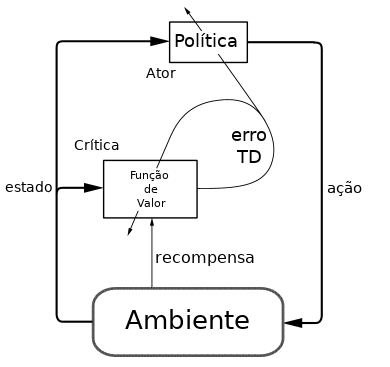
\includegraphics[width=10cm]{imagens/actor-critic_portuguese.png}}
\small{Fonte: Autor}
\label{fig:actor_critic}
\end{figure}

\subsection{Aprendizado por Reforço Profundo}

O objetivo do Aprendizado por Reforço Profundo (Deep-RL) é controlar um agente na tentativa de maximizar sua função de recompensa.
O algoritmo \textit{Deep Q-Network} \cite{mnih2013playing} foi capaz de desempenhar em nível humano muito dos jogos eletrônicos do Atari por fazer a estimativa das ações de um agente.
Contudo, enquanto a DQN pode resolver problemas em espaços de observações complexos, ela pode apenas lidar com espaços de ações discretos.
E é notável que muitas tarefas, no controle da robótica, têm espaços de ações contínuos.
Então DQN não podem ser aplicadas em domínios contínuos e é necessário usar outros algoritmos capazes de lidar com esse tipo de problema.

\subsubsection{Política de Gradiente Determinística Profunda}

O algoritmo de política de gradiente determinística profunda (DDPG) consiste de um método ator-críticab de política-\textit{off} que usa funções de aproximação que pode aprender políticas de espaço de ação contínuo.
O algoritmo faz uso de uma rede neural para a rede ator e outro para a rede crítica.
Essas duas redes computam a predição de ação para o estado atual e geram um sinal de erro de diferença temporal para cada intervalo de tempo.
A entrada da rede ator é o estado atual, e a saía é um valor real que representa uma ação escolhida para um espaço contínuo de ação.
A saída da crítica é simplesmente o valor de Q estimado do estado atual e ação dada pelo ator.

O maior desafio do aprendizado em espaço de ações contínuas é a exploração. 
Para enfrentar esse desafio é preciso construir a política de exploração $\mu'$ pela adição da amostra de ruído de um processo de ruído $\mathcal{N}$ para a política da rede ator, que é definida como:
\begin{equation}
    \mu' = \mu(s_t) + \mathcal{N}
\end{equation}

Onde $\mathcal{N}$ pode ser escolhido de um jeito que se adéqua ao ambiente. Sendo o processo de Ornstein-Uhlenbeck \cite{uhlenbeck1930theory} o mais usado para gerar eficiência de exploração correlacionada temporalmente em problemas de controle físico.

Em geral, treinar e avaliar a função de política que sai da rede ator e a função de valor que sai da rede crítica, com milhares de trajetórias simuladas correlacionadas temporalmente, leva a introdução de enormes quantidades de variância na aproximação da função verdadeira Q (crítica).
É sugerido usar uma memória de repetição para armazenar as experiências do agente durante o treino \cite{schaul2015prioritized}. 
Isto é, salvar os estados, ações, recompensas e novos estados que o agente explorou durante o episódio.
E então, aleatoriamente selecionar as experiências que vão ser usadas no aprendizado, para assim, quebrar a correlação temporal com os diferentes episódios dos treinos.

A experiência de repetição permite ao agente inteligente aprender de memórias recentes, fazendo com que aumente a velocidade de aprendizado e a quebra de correlações temporais indesejadas. Mesmo com a aplicação de uma memória curta é possível ver uma melhora substancial na desempenho do agente. 
Apesar da aplicação de uma memória de repetição deixar mais lento o aprendizado do agente, se consegue um melhor desempenho dele.

Sem contar a utilização da memória de repetição é preciso fazer uma rede alvo para gerar alvos para que o erro da diferença temporal possa ser regularizado no aprendizado do algoritmo e aumentar a estabilidade. 
A rede alvo é uma rede que possui uma cópia da rede ator e da rede crítica, porém, a sua atualização é feita de um modo “leve”.
Isso quer dizer que a rede alvo não copia diretamente os pesos da rede ator e da rede crítica. 
Os pesos, representado por $\theta$, da rede alvo são atualizados deste modo:
\begin{equation}
    \theta' \leftarrow \tau \theta + (1+\tau)\theta'
\end{equation}

Com $\tau \ll 1$ . Onde o alvo é representado pela apóstrofe.
Então o valores do alvo da rede mudam de forma lenta e assim permitem uma melhora da estabilidade do treinamento.

O algoritmo DDPG é descrito no Algoritmo \ref{alg:ddpg}. Nesta definição é possível ver com mais clareza o algoritmo de aprendizado por reforço profundo. Demonstrando toda etapa de treinamento da rede ator e da rede crítica.

% \begin{algorithm}
% \caption{DDPG com repetição de memória}
% \label{alg:ddpg}
% \begin{algorithmic}
% \STATE Aleatoriamente inicializa a rede crítica $Q(s,a|\theta^Q)$ e a rede ator $\mu(s|\theta^{\mu})$ com os pesos da rede $\theta^Q$ e $\theta^\mu$
% \STATE Inicializa a rede alvo $Q'$  e $\mu'$ com pesos $\theta^{Q'} \leftarrow \theta^Q$, $\theta^{\mu'} \leftarrow \theta^{\mu}$
% \STATE Inicializa a memória de repetição $R$
% \FOR{episódio = 1 até M}
% \STATE Inicializa um processo aleatório $\mathcal{N}$ para a ação de exploração
% \STATE Recebe o estado de observação $s_1$
% \FOR{t = 1 até T}
% \STATE Seleciona a ação $a_t = \mu(s_t|\theta^{\mu})+\mathcal{N}_t$ de acordo com a política atual e ruído de\\ exploração
% \STATE Executa a ação $a_t$ e observa a recompensa $r_t$ e observa o novo estado $s_{t+1}$
% \STATE Armazena a transição $(s_i,a_i,r_i,s_{i+1})$ em $R$
% \STATE Retira um \textit{minibatch} de amostras aleatórias de $N$ transições $(s_t,a_t,r_t,s_{t+1})$ de $R$
% \STATE Define $y_i = r_i + \gamma Q'(s_{i+1}, \mu'(s_{i+1}|\theta^{\mu'})|\theta^{Q'})$
% \ENDFOR
% \ENDFOR
% \end{algorithmic}
% \end{algorithm}

\vspace{1.5cm}
\begin{algorithm}[H]
\DontPrintSemicolon
Aleatoriamente inicializa a rede crítica $Q(s,a|\theta^Q)$ e a rede ator $\mu(s|\theta^{\mu})$ com os pesos da rede $\theta^Q$ e $\theta^\mu$. \;
Inicializa a rede alvo $Q'$  e $\mu'$ com pesos $\theta^{Q'} \leftarrow \theta^Q$, $\theta^{\mu'} \leftarrow \theta^{\mu}$. \;
Inicializa a memória de repetição $\mathcal{R}$.\;
\Para{episódio = 1 até M}{
Inicializa um processo aleatório $\mathcal{N}$ para a ação de exploração. \;
Recebe o estado de observação $s_1$.\;
\Para{t = 1 até T}{
Seleciona a ação $a_t = \mu(s_t|\theta^{\mu})+\mathcal{N}_t$ de acordo com a política atual e ruído de exploração.\;
Executa a ação $a_t$ e observa a recompensa $r_t$ e observa o novo estado $s_{t+1}$.\;
Armazena a transição $(s_t,a_t,r_t,s_{t+1})$ em $\mathcal{R}$.\;
Retira um \textit{minibatch} de amostras aleatórias de $N$ transições $(s_i,a_i,r_i,s_{i+1})$ de $\mathcal{R}$.\;
Define $y_i = r_i + \gamma Q'(s_{i+1}, \mu'(s_{i+1}|\theta^{\mu'})|\theta^{Q'})$. \;
Atualiza a rede crítica minimizando a perda: $L = \frac{1}{N} \sum_{i} (y_i - Q(s_i,a_i | \theta^Q ))^2$.\;
Atualiza a política da rede ator usando o gradiente de política da amostra retirada:\;
\begin{equation*}
    \nabla_{\theta^\mu}J  \approx  \frac{1}{N} \sum_{i} \nabla_a Q( s,a | \theta^Q ) |_{ s=s_i, a=\mu(s_i) } \nabla_{\theta^\mu}\mu( s | \theta^\mu ) |_{s_i}
\end{equation*}
Atualiza a rede alvo:
\begin{gather*}
    \theta^{ Q' } \leftarrow  \tau\theta^Q + ( 1+\tau )\theta^{ Q' }\\
    \theta^{ \mu' } \leftarrow  \tau\theta^\mu + ( 1+\tau )\theta^{ \mu' }
\end{gather*}
}
}
\caption{DDPG com repetição de memória}
\label{alg:ddpg}
\end{algorithm}
\vspace{1.0cm}

% Para melhor que representar o algoritmo, na Figura 4, foi feito um fluxograma de forma a representar o treino da rede DDPG.
% Quando o treino começa as redes crítica, ator e alvo são inicializadas de forma aleatória. 
% O treino dura no total M episódios, onde cada episódio tem T intervalos.

% \begin{figure}[H]
% \caption{Flosefes}
% \centerline{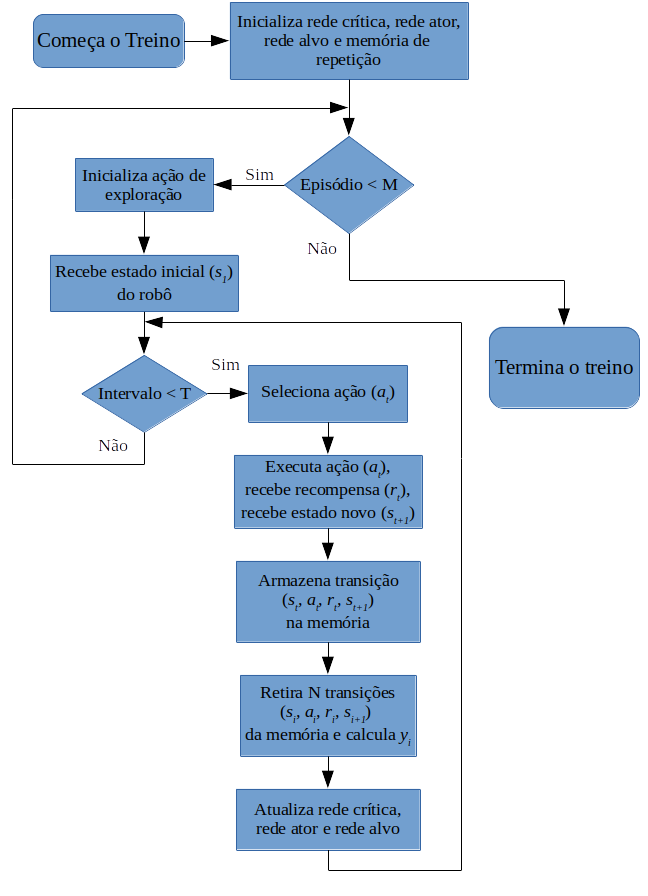
\includegraphics[width=10cm]{imagens/flowchart_ddpg.png}}
% \small{Fonte: Autor}
% \label{fig:flowchart_ddpg}
% \end{figure}

\subsubsection{Ator-Crítica Suave (SAC)}

O Ator-Crítica Suave (SAC) é um algoritmo que otimiza uma política estocástica de um modo de política-\textit{off}. A rede consiste de um método ator-crítica que usa funções de aproximação que podem aprender políticas de ação em espaços contínuos \cite{haarnoja2018soft}.
O algoritmo faz uso de uma rede neural para a rede ator, a rede valor de $V$, e outra para rede crítica.
Essas 3 redes computam a predição de ação para o estado atual e gera um sinal de erro de diferença temporal para cada intervalo de tempo.

A característica central do SAC é a regularização de entropia.
Ao invés de apenas procurar a maximização da recompensa do sistema, a SAC procura também maximizar a entropia da política.
O aumento da entropia resulta é um agente que pode explorar melhor seu ambiente, o que ajuda no aprendizado. E pode prevenir também com que uma política convirja muito cedo para um política local ótima.

A entropia se refere ao quão imprevisível uma variável aleatória pode ser.
Então, se uma variável sempre toma um único valor isso quer dizer que a entropia é considerada zero pois não é nenhum pouco imprevisível.
Uma entropia alta na política explicitamente encoraja a exploração do agente pois é atribuído uma probabilidade igual para a ação que tem o mesmo ou igual valor de $Q$ e assegura que não seja colapsado em repetidamente selecionar uma ação particular do agente.

Para calcular a entropia de $\mathcal{H}$ de uma variável aleatória $x$ de função de densidade $P$, é possível através de:
\begin{equation}
    \mathcal{H}(P) = \mathbb{E}_{x \sim P} [-\log P(x)]
\end{equation}

A rede SAC utiliza dos mesmos métodos de repetição de memória e de uma rede alvo que a rede DDPG. No Algoritmo \ref{alg:sac} é mostrado as etapas de treinamento da rede ator, da rede crítica e da rede de valor $V$ no SAC.

\vspace{1.5cm}
\begin{algorithm}[H]
\DontPrintSemicolon
Aleatoriamente inicializa a rede crítica $Q(s,a|\theta^{Q_{1}})$, $Q(s,a|\theta^{Q_{2}})$, a rede ator $\pi(s,a|\theta^{\pi})$ e a rede de valor de $V(s|\theta^V)$ com os pesos da rede $\theta^{Q_1}$, $\theta^{Q_2}$, $\theta^\pi$ e $\theta^V$. \;

Inicializa a rede alvo $V'$com pesos $\theta^{V'} \leftarrow \theta^V$\;
Inicializa a memória de repetição $\mathcal{R}$.\;

\Para{episódio = 1 até M}{
Recebe o estado de observação $s_1$.\;

\Para{t = 1 até T}{
Seleciona a ação $a_t \sim \pi(s_t,a_t|\theta^{\pi})$ de acordo com a política atual.\;

Executa a ação $a_t$ e observa a recompensa $r_t$ e observa o novo estado $s_{t+1}$.\;

Armazena a transição $(s_t,a_t,r_t,s_{t+1})$ em $\mathcal{R}$.\;

Retira um \textit{minibatch} de amostras aleatórias de $N$ transições $(s_i,a_i,r_i,s_{i+1})$ de $\mathcal{R}$.\;

Computa os alvos para a rede ator $Q$ e  $V$:
\begin{gather*}
    y_q(r_i, s_{i+1}) =  r_i + \gamma V(s_{i+1}|\theta^{V'})
    \\
    y_v (s_i) = \min_{k=1,2} Q(s_i, a_i|\theta^{Q_k}) - \alpha \log \pi (s_i, a_i|\theta^{\pi})
\end{gather*}

Atualiza a rede crítica usando o gradiente
\begin{equation*}
    \nabla_{\theta^Q_k} \frac{1}{|B|} \sum_{(s_i,a_i,r_i,s_{i+1}) \in B} (Q(s_i, a_i|\theta^{Q}_k) - y_q(r_i, s_{i+1}))^2 \qquad \textrm{for}\: k = 1,2 
\end{equation*}

Atualiza a rede valor de $V$ usando o gradiente
\begin{equation*}
    \nabla_{\theta^V} \frac{1}{|B|} \sum_{s_i \in B} (V(s_i|\theta^V) - y_v(s_i))^2
\end{equation*}

Atualiza a política da rede ator usando o gradiente
\begin{equation*}
    \nabla_{\theta^\pi} \frac{1}{|B|} \sum_{s_i \in B} (Q(s_i, a_i|\theta^{\pi}) - \alpha \log \pi (s_i, a_i|\theta^{\pi}))
\end{equation*}

Atualiza a rede valor de $V$ alvo com
\begin{gather*}
    \theta^{ V' } \leftarrow  \tau\theta^V + ( 1+\tau )\theta^{ V' }
\end{gather*}
}
}
\caption{SAC com repetição de memória}
\label{alg:sac}
\end{algorithm}
\vspace{1.0cm}

\section{Visão Computacional}

A visão computacional é ciência da computação e sistemas de \textit{software} que podem reconhecer e entender uma imagem ou cena \cite{forsyth2002computer}.
A visão computacional também é composta de vários aspectos tais como reconhecimento de imagem, detecção de objetos geração de imagem, super-resolução de imagem e mais.
Do ponto de vista da engenharia, ela procura automatizar tarefas que o sistema visual humano pode fazer.
A detecção de objetos é provavelmente o mais profundo aspecto da visão computacional devido ao grande número de casos práticos.

\subsection{Rastreamento de Objetos}

Para fazer o rastreamento de objetos primeiramente é preciso detectar um objeto.
A detecção de objetos se refere a capacidade de computadores e sistemas de \textit{software} de localizar em um imagem ou cena e de identificar cada objeto.
Sendo amplamente utilizado para detecção de faces, detecção de veículos, pedestres e carros autônomos.
Existem muitas maneiras que a detecção de objetos pode ser usada. Em muitos casos a cor do objeto é usado para sua detecção.

O rastreamento de objetos é o processo de localizar um objeto alvo movendo em quadros consecutivos de um vídeo \cite{bascle1995region}. Essa associação pode ser especialmente difícil quando o objeto se move rápido em relação a taxa de quadros do vídeo. Outra situação que aumenta a complexidade do problema é quando o objeto rastreado se move em relação ao tempo. Para essas situações geralmente são aplicados modelos de movimento em que é descrito como a imagem do alvo pode mudar para diferente movimentos dos objetos. Essas aplicações se encontram muito relacionadas com a robótica. Já que muitas aplicações usam de visão para poder completar suas tarefas.
\chapter{Materiais e Métodos}

Para o análise de uma rede SAC e DDPG foram usado a linguagem de programação Python.
A linguagem Python tem como prioridade a legibilidade do código sobre a velocidade \cite{ascher1999learning}. 
As vastas bibliotecas e \textit{frameworks} proporcionados pelo Python faz dela uma ferramenta extraordinária para fins de aprendizado de máquina e análise de dados.

\section{ROS}

O sistema operacional de robôs (ROS) é uma \textit{framework} flexível para escrever \textit{software} para robôs.
o ROS \cite{pyo2015ros} é uma coleção de ferramentas e bibliotecas.
O ROS fornece serviços padrões de sistemas operacionais, tais como a abstração de \textit{hardware}, controle de dispositivos de baixo nível, mensagens entre processos e gerenciamento de pacotes.
O conjunto de processos do ROS execução são representados em arquitetura de grafos onde o processamento é realizado em nós que recebem e enviam mensagens como sensores, controle, estado, planejamento, atuador e outros.

Apesar da importância da baixa latência no controle de robôs, o ROS não é um sistema operacional em tempo real, embora seja possível integrar o ROS com códigos em tempo real. Essa falta do sistema de tempo real está sendo endereçada no desenvolvimento do ROS 2.0.

\section{Gazebo}

A simulação de robôs é uma ferramenta essencial em toda a caixa de ferramentas de um roboticista.
Um bom simulador faz possível se testar rapidamente algoritmos, desenhar robôs, e treinar sistemas com inteligência artificial usando cenários realistas.
Com o Gazebo \cite{fairchild2016ros} é possível simular estes ambientes facilmente e com a vantagem de ter uma comunidade ativa. Isso faz do Gazebo uma grande ferramenta na área de simulação de robótica. Na Figura \ref{fig:gazebo} é mostrado a simulação do robô Turtlebot3 Burger em um ambiente de 3D no simulador Gazebo.

\begin{figure}[H]
\caption{Turtlebot3 Burger na simulação do Gazebo}
\centerline{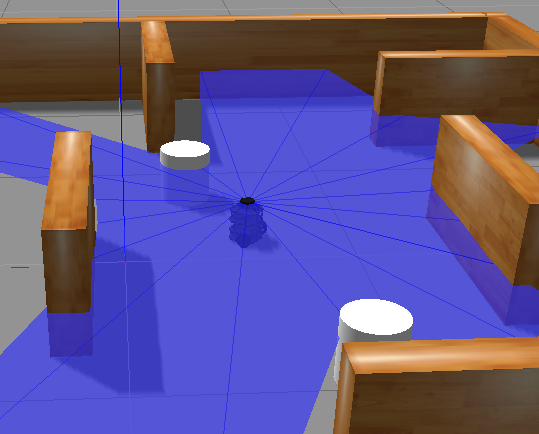
\includegraphics[width=\columnwidth]{imagens/gazebo.png}}
\small{Fonte: Autor}
\label{fig:gazebo}
\end{figure}

\section{Turtlebot}

O Turtlebot é uma robô de plataforma padrão ROS, e existem 3 versões da série.
Os Turtlebots são robôs móveis acessíveis e programáveis para o uso na educação, pesquisa, e \textit{hobbies} e prototipagem de produtos. A terceira versão foi usada no projeto e é mostrada na Figura \ref{fig:burger}.

\begin{figure}[H]
\caption{Turtlebot3 Burger real e simulado no Gazebo}
\centerline{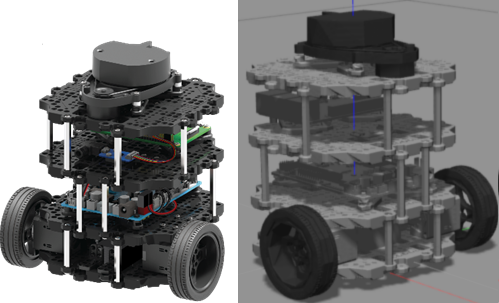
\includegraphics[width=\columnwidth]{imagens/burger.png}}
\small{Fonte: \cite{robotisemanual}}
\label{fig:burger}
\end{figure}

O Turtlebot3 Burger usa 2 motores DYNAMIXEL da série XL, para a detecção de objetos o Turtlebot3 utiliza um sensor \textit{laser} 360$^{\circ}$ LiDAR, e uma unidade de medição inercial (IMU) para o cálculo da odometria.
Todo o controle é feito pela placa controladora de código aberto OpenCR1.0 e o microprocessador Raspberry Pi 3.
A Tabela \ref{tab1} mostra todas as especificações de \textit{hardware} do Turtlebot3 versão Burger.

\begin{table}[H]
\caption{Especificação de Hardware do Turtlebot3 Burger}
\begin{center}
\begin{tabular}{l|l}
\hline
\textbf{Itens}&\textbf{Especificação} \\
\hline
Velocidade translacional máxima & 0.22 m/s \\
\hline
Velocidade rotacional máxima   & 2.84 rad/s (162.72$^{\circ}$/s) \\
\hline
Carga máxima                & 15kg \\ 
\hline
Tamanho (L x W x H)               & 138mm x 178mm x 192mm \\
\hline
Peso                        & 1kg \\
\hline
Limiar de escalada          & 10 mm ou mais baixo \\
\hline
Tempo de operação esperado       & 2h 30m \\
\hline
Tempo de espera para carregamento         & 2h 30m \\
\hline
Computador de Placa Única (SBC)   & Raspberry Pi 3 Model B e B+ \\
\hline
Atuador                       & DYNAMIXEL XL430-W250 \\
\hline
Sensor de Distância \textit{Laser} (LDS)     & 360 LDS-01 \\
\hline
IMU                            & \begin{tabular}[l]{@{}l@{}}Giroscópio 3 eixos\\ Acelerômetro 3 eixos\\ Magnetômetro 3 eixos\end{tabular} \\
\hline
Bateria                        & \begin{tabular}[l]{@{}l@{}}Polímero de lítio \\ 11.1V 1800mAh / 19.98Wh 5C \\ \end{tabular} \\
\hline

\end{tabular}
\label{tab1}
\end{center}
\small{Fonte: Adaptado de \cite{robotisemanual}}
\end{table}

\section{OpenCV}

\textit{Open Source Computer Vision} (OpenCV) é uma biblioteca de \textit{software} de código aberto para visão computacional e aprendizagem de máquina.
É principalmente usada para o desenvolver aplicações avançadas para processamento de imagem e visão compuacional (\citeauthor{bradski2008learning}, \citeyear{bradski2008learning}; \citeauthor{wang2010camera}, \citeyear{wang2010camera}).
OpenCV pode tirar quadros de um vídio e executar algoritmos para pegar informações necessárias.
Pode também identificar um objeto, reconhecer uma face ou rastrear o movimento de um objeto.
É comumente usado em aplicações de robótica \cite{oyama2009come}.

\section{Ambientes de Simulação}

Foram usados três ambientes para as simulações.
O primeiro ambiente é mostrado na Figura \ref{subfig:simulated_env1}, o ambiente representa uma área livre para o robô se mover.
As paredes do ambiente são as únicas coisas onde o agente pode colidir.
Se o robô móvel colidir com a parede ou qualquer obstáculo, uma recompensa negativa é dada para esta ação e o episódio atual termina.
O segundo ambiente é mostrado na Figura \ref{subfig:simulated_env2} e tem quatro obstáculos fixos.
Isso significa que este ambiente é mais complexo de um modo que o agente inteligente tem que fazer uma melhor estratégia para não colidir.
O terceiro ambiente, mostrado na Figura \ref{subfig:simulated_env3}, é mais complexo que os ambientes anteriores.
O número de paredes e obstáculos móveis, representados pelos blocos brancos, fazem o ambiente mais dinâmico, se aproximando de um ambiente no mundo real.

\begin{figure}[H]
\caption{Ambientes de treinamento usados na simulação do Gazebo}
    \begin{center}
    \begin{subfigure}[b]{0.3\textwidth}
        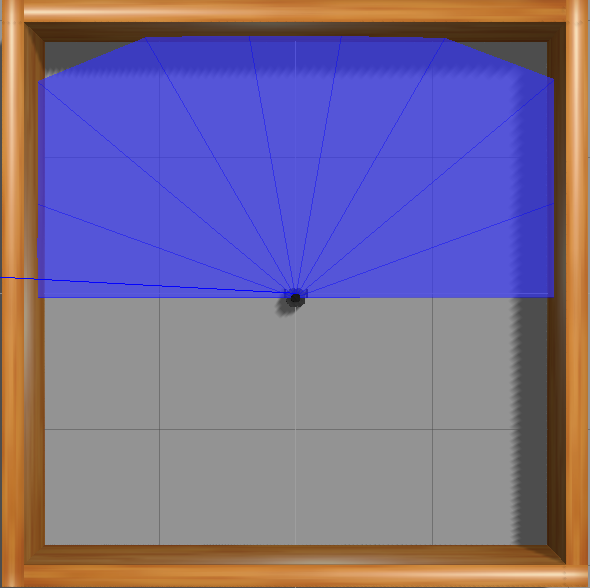
\includegraphics[width=\textwidth]{imagens/simulated_envs/amb1.png}
        \caption{Primeiro ambiente}
        \label{subfig:simulated_env1}
    \end{subfigure}
    ~ %add desired spacing between images, e. g. ~, \quad, \qquad, \hfill etc. 
      %(or a blank line to force the subfigure onto a new line)
    \begin{subfigure}[b]{0.3\textwidth}
        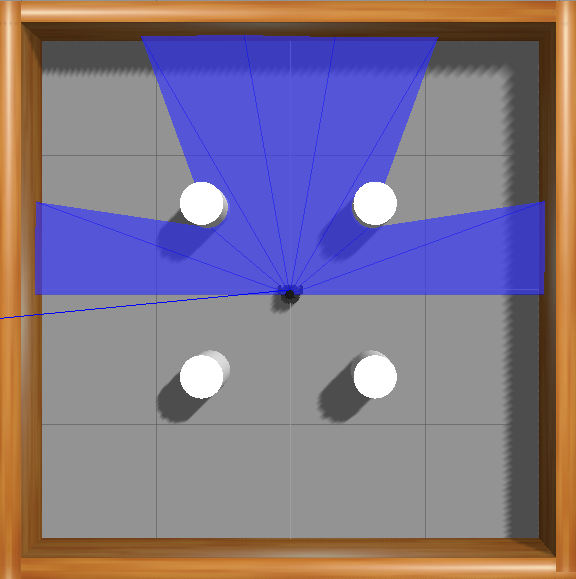
\includegraphics[width=\textwidth]{imagens/simulated_envs/amb2.png}
        \caption{Segundo ambiente}
        \label{subfig:simulated_env2}
    \end{subfigure}
    ~ %add desired spacing between images, e. g. ~, \quad, \qquad, \hfill etc. 
      %(or a blank line to force the subfigure onto a new line)
    \begin{subfigure}[b]{0.3\textwidth}
        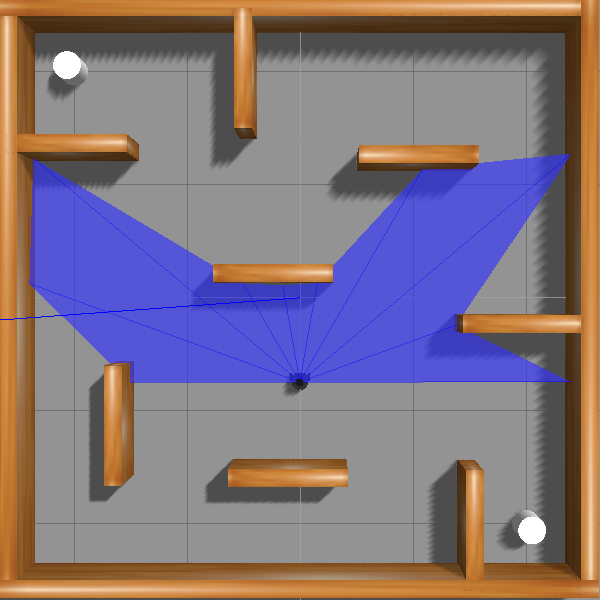
\includegraphics[width=\textwidth]{imagens/simulated_envs/amb3.png}
        \caption{Terceiro ambiente}
        \label{subfig:simulated_env3}
    \end{subfigure}\label{fig:environments}
    \end{center}
\small{Fonte: Autor}
\end{figure}

\section{Ambientes real}

Depois de treinar a rede DDPG e rede SAC por simulação, as redes serão testadas em um cenário real.
O Turtlebot3, versão Burger, será utilizado para executar estes testes.
Algumas das entradas necessárias das redes no ambiente real foram obtidas por processamento de imagem.
O primeiro ambiente real é mostrado na Figura \ref{subfig:real_env1} e se assemelha com o primeiro ambiente de simulação sem obstáculos.
O segundo ambiente real é mostrado na Figura z\ref{subfig:real_env2} e ele apresenta um ambiente complexo similar ao segundo e terceiro ambiente usado em simulação.

\begin{figure}[H]
\caption{Ambientes criados para testes da rede DDPG e rede SAC em ambiente real}
    \begin{center}
    \begin{subfigure}[b]{0.45\textwidth}
        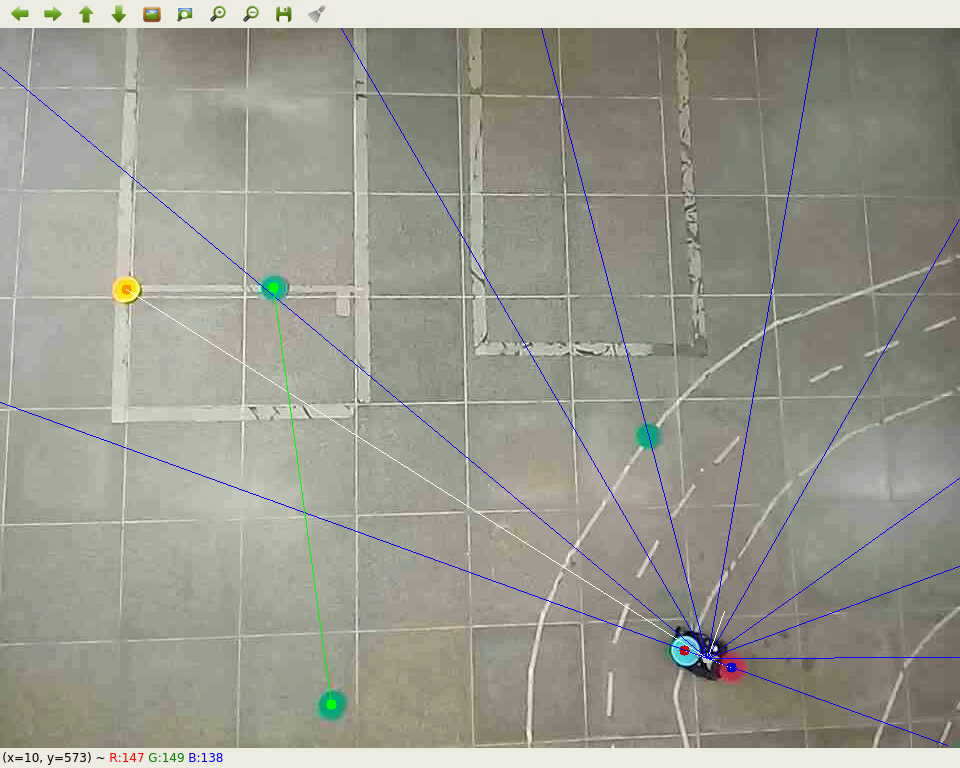
\includegraphics[width=\textwidth]{imagens/real_env1.png}
        \caption{Primeiro ambiente real}
        \label{subfig:real_env1}
    \end{subfigure}
    ~
    \begin{subfigure}[b]{0.45\textwidth}
        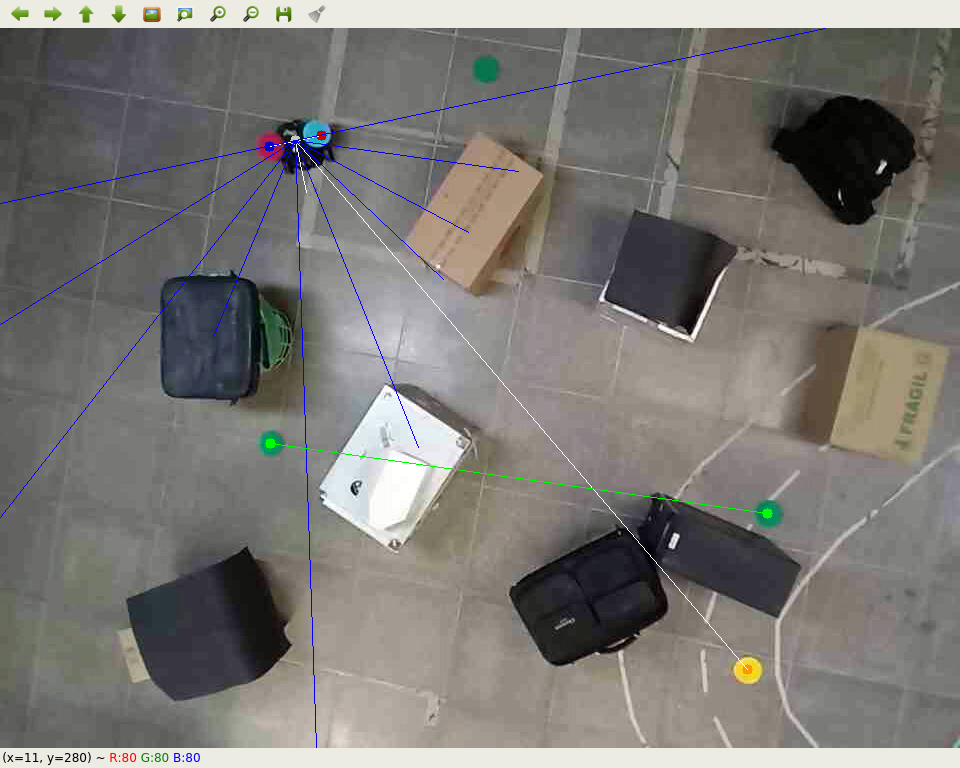
\includegraphics[width=\textwidth]{imagens/real_env2.png}
        \caption{Segundo ambiente real}
        \label{subfig:real_env2}
    \end{subfigure}
    \end{center}
    \label{fig:real_environments}
\small{Fonte: Autor}
\end{figure}

\section{Métodos}

A intenção deste trabalho é propor um sistema para um robô móvel em ordem de planejar seu movimento sem qualquer conhecimento do mapa no ambiente. Sua função de transição é definida como:
\begin{equation}
    v_t = f(x_t, p_t, v_{t-1})
\end{equation}

Onde $x_t$ é a observação da informação bruta do sensor, $p_t$ é a posição relativa do alvo em coordenadas polar, e $v_{t-1}$ é a velocidade do robô móvel no último intervalo de tempo.
Todas variáveis especificadas, anteriormente, podem ser definidas como o estado atual $s_t$ do robô móvel.
Na Figura \ref{fig:state_action} é mostrado o sistema de estados e ações que será utilizado nas redes para o treinamento.
Com esse modelo é possível retirar a ação que o robô fará, dado o seu estado atual.
Contudo, é preciso assegurar a frequência mínima de leitura dos dados de entrada para controlar o movimento do robô.
Pois se o robô tem uma leitura de frequência lenta das entradas, ele não pode reagir à um obstaculo na trajetória até o alvo.
Desde jeito, o robô pode reagir a novos estados rapidamente.
Esse método foi primeiro explorado por \cite{tai2017virtual}.

\begin{figure}[H]
\caption{Sistema de estados e ações}
\centerline{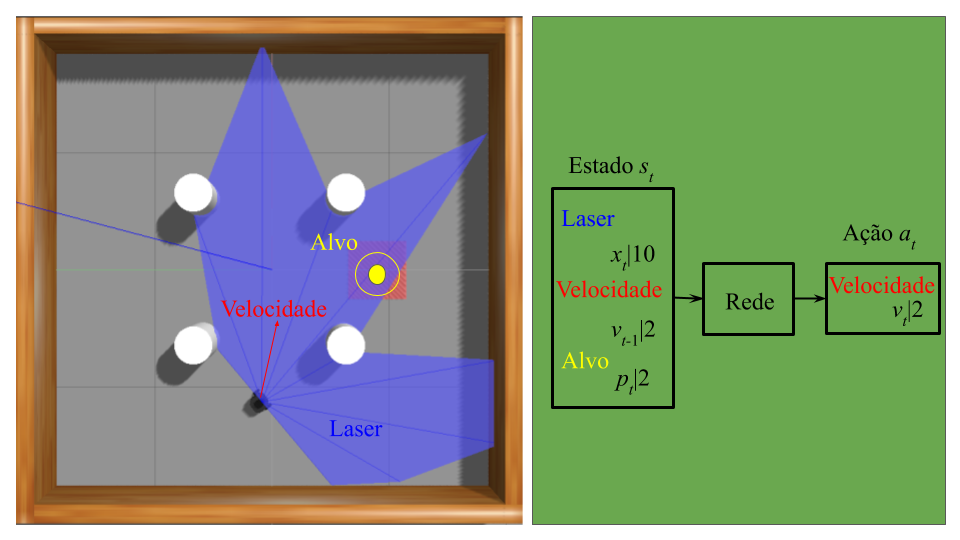
\includegraphics[width=\columnwidth]{imagens/state_action.png}}
\small{Fonte: Autor}
\label{fig:state_action}
\end{figure}

\subsection{Estruturas das Redes}

Uma vez que os sistema de estados e ações tenham sido definidos, é possível criar uma rede DDPG ou SAC para resolver o problema.
As redes têm como 14 entradas, como apresentado na Figura \ref{fig:in_out}, no qual 10 correspondem às leituras do \textit{laser} $x_t$, 2 correspondem à velocidade anterior linear $v_{t-1}$ e angular $\omega_{t-1}$, e 2 correspondem a posição relativa $d_t$ e ângulo $\theta_t$ do robô móvel ao alvo.
As amostras da leitura do sensor \textit{laser} são entre $-$90$^\circ$ e 90$^\circ$ em relação ao robô. A saída da rede é a ação de velocidade linear $v_t$ e angular $\omega_t$ que são aplicadas no robô móvel.

\begin{figure}[H]
\caption{Entradas e saídas da rede}
\centerline{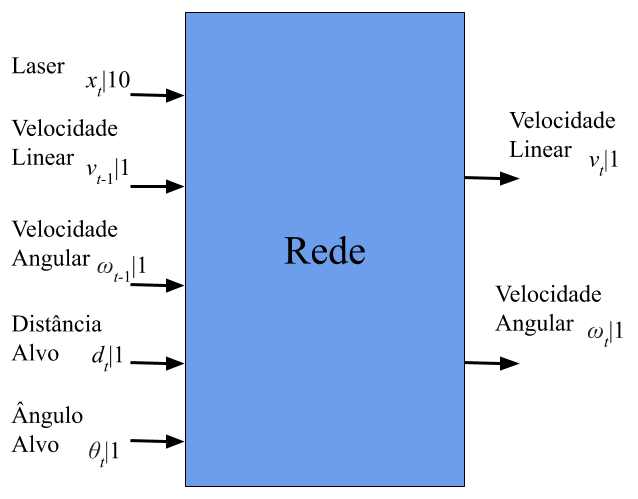
\includegraphics[width=10cm]{imagens/input_and_output.png}}
\small{Fonte: Autor}
\label{fig:in_out}
\end{figure}

A estrutura da rede DDPG é mostrada na Figura \ref{fig:ddpg_struct}. A rede ator tem como entrada o estado atual do robô móvel seguida por 3 camadas de redes neurais totalmente conectadas com 512 neurônios. A entrada da rede é transformada na velocidade linear e angular que serão os comandos enviados para os motores do robô móvel.
O intervalo da velocidade angular está restringindo entre $(-1,1)$ e a função de tangente hiperbólica $(tanh)$ é usada como função de ativação.
O intervalo da velocidade angular usou da função sigmóide como função de ativação para restringir a seus valores entre $(0,1)$.
Como não há leituras do sensor \textit{laser} na parte de trás do robô, a movimento de deslocamento de ré não é necessário.
As ações de saídas são então multiplicadas com os dois
hiperparâmetros que decidem a velocidade final linear e angular executada pelo robô móvel.
Para isso, foi usado como velocidade máxima linear $0.22$ $m/s$ e velocidade máxima angular $2$ $rad/s$ no robô Turtlebot3 versão Burger.
Na rede crítica, o valor de $Q$ do estado e ação atual são previstos.
Usando apenas 3 camadas de redes neurais totalmente conectadas para processar a entrada. Onde a ação, saída da rede ator, é concatenada na segunda camada de rede neural.
O valor de $Q$ é ativado através de uma função de ativação linear simples. Todas as respostas das funções de ativação citadas são mostradas na Figura \ref{fig:FA}.

\begin{figure}[H]
\caption{Estrutura do modelo da rede DDPG}
\centerline{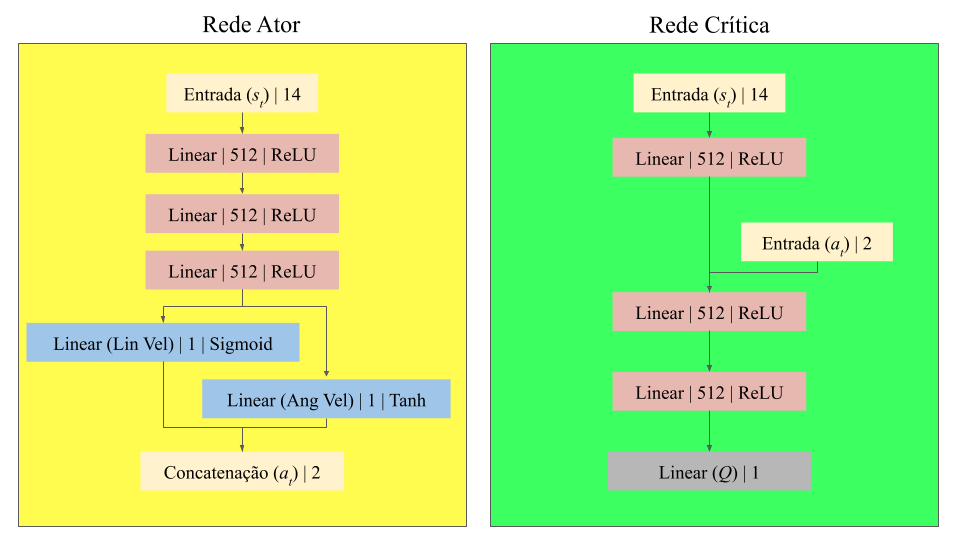
\includegraphics[width=\columnwidth]{imagens/ddpg_structure.png}}
\small{Fonte: Autor}
\label{fig:ddpg_struct}
\end{figure}

A estrutura da rede SAC é mostrada na Figura \ref{fig:sac_struct}.
A saída da rede ator tem o estado atual do robô móvel seguido por 4 camadas de redes neurais totalmente conectadas com 512 neurônios.
A entrada da rede é transformada nos comandos de velocidade angular e linear enviados para o robô móvel, do mesmo jeito que ocorre na rede ator da DDPG.
O intervalo de ação é restringindo entre $(-1,1)$ pela função de ativação de tangente hiperbólica. 
E as saídas da ação são mudados para a velocidade linear que varia entre $0$ até $0.22$ $m/s$ e a velocidade angular é entre $-2$ até $2$ $rad/s$ no Turtlebot3.
Já como diferença da rede DDPG, a rede SAC apresenta uma rede crítica que prediz o valor de $Q$ e uma rede de valor $V$ que prediz o valor do estado atual.
As duas redes usam apenas 2 camadas totalmente conectadas para processar o estado de entrada.

\begin{figure}[H]
\caption{Estrutura do modelo da rede SAC}
\centerline{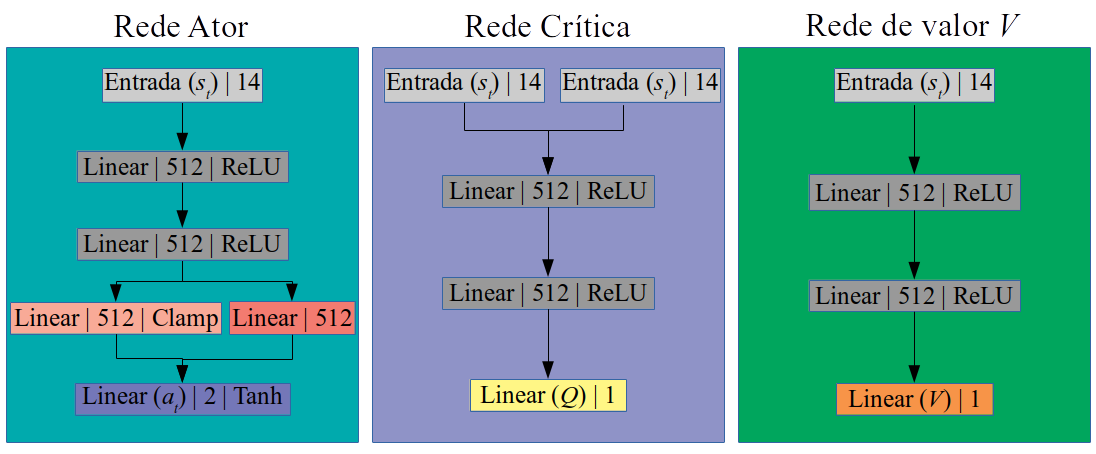
\includegraphics[width=\columnwidth]{imagens/sac_structure.png}}
\small{Fonte: Autor}
\label{fig:sac_struct}
\end{figure}

\subsection{Função de Recompensa}

Uma vez que o ambiente seja definido, é possível simular um robô móvel controlado para a tarefa de navegação.
É necessário definir o sistema recompensa e penalidade para a rede DDPG e SAC.
Lembrando que as recompensas e penalidades são números atribuídos passados para o agente inteligente.
Através disso, a rede vai fazer a propagação desses dados para seus pesos e bias em ordem para aprender os hiperparâmetros.

Existem quatro diferente condições para o sistema de recompensa que apresentaram melhores resultados para a resolução do problema e são os seguintes:

\begin{equation}
r (s_t, a_t) = 
\begin{cases}
r_{alcan\textit{ç}a} \ \textrm{se} \ d_t < c_d
\\
r_{colis\tilde{a}o} \ \textrm{se}\ min_x < c_o
\\
c_{r1}(d_{t-1} - d_t) \ \textrm{se} \ (d_{t-1} - d_t) > 0
\\
c_{r2} \ \textrm{se} \ (d_{t-1} - d_t) \leq 0
\end{cases}
\label{eq:r_function}
\end{equation}

Na Equação \ref{eq:r_function}, se o robô chega ao algo através da verificação de limite de distância $c_d$, uma recompensa positiva $(r_{alcan\textit{ç}a})$ é dada, mas se o robô colidir com um obstáculo através da verificação das leituras de alcance mínimo, uma recompensa negativa $(r_{colis\tilde{a}o})$ é dada.
Ambas as condições são suficientes para terminar o episódio de treino.
Ao contrário disso, a recompensa é baseada na diferença de distância do alvo comparado ao último intervalo de tempo $(d_{t-1} - d_t)$.
Se essa diferença é positiva a recompensa dada é a distância percorrida multiplicada pelo hiperparâmetro $(c_{r1})$, e se a a distância é negativa é usado o hiperparâmetro $(c_{r2})$.
Isso motiva o robô móvel a chegar mais próximo à posição do alvo e encoraja o agente a evitar obstáculo no ambiente.

\subsection{Positioning capture in real environments}

% % 
% % 
% % 
% estoy aqyu%%%%%%%%

After training the DDPG network through simulation, it will be tested in a real scenario.
The Turtlebot3, version Burger, will be used to perform this test.
It will be necessary to obtain the angle and distance of a target for the network to complete its goal.
So it was setup a camera in the ceiling to extract this information.

Firstly, the essential points positions to extract the angle and distance are taken from the image.
These positions include the target, left and right side of the robot, and three points to be a distance reference parameter.
Figure \ref{fig:pixel_to_meter} shows a frame of the scenario in which there were used different colored circles to identify the relevant points.
The yellow circle was attached as the target, the blue to the left side of the robot, the red to the right side and the three green circles were used as reference parameter to calculate the distance.

\begin{figure}[H]
\centerline{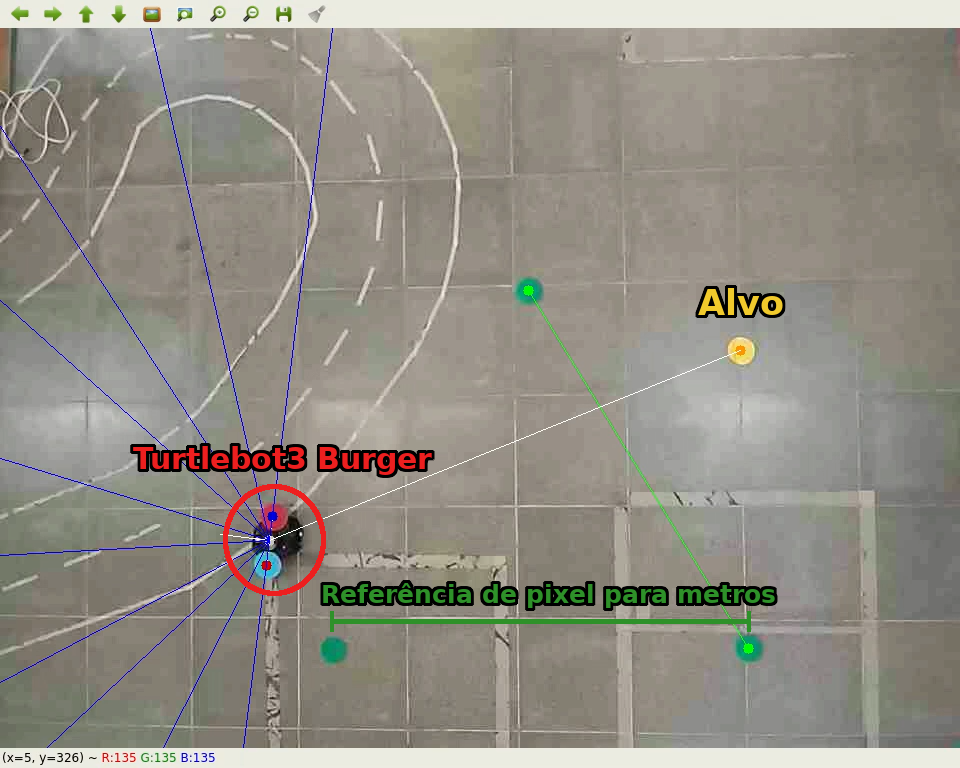
\includegraphics[width=10cm]{imagens/pixel_to_meter.png}}
\caption{Real environment relevant points}
\label{fig:pixel_to_meter}
\end{figure}


After the points were extracted from the center of the circles, it is possible to calculate the two necessary DDPG network inputs.
So, it is necessary to figure out the vector distance that connects the center of the Turtlebot3 to the target point, and the vector direction which represents the direction of the robot.
% Firstly, it is needed to compute the vector $distance$.
% It starts from the center of the Turtlebot3, which is equal to the midpoint of the blue and red points.
% The center of green circles have a predefined distance from each other, that helps to calculate the robot and target distance, doing by converting the module of vector $distance$ in pixels to the distance in meters.
% In other words, the actual distance between target and robot is estimated by comparing the pixels of the norm of the vector $distance$ with the pixels from the norm of the vector that connects the green circles, which real distance is already known. 
% %direction vector   
% The vector $direction$, like the $distance$, starts from the center of the Turtlebot3.
% With the blue and red circles that are on left and right sides of the mobile robot, respectively, it is possible to determine the direction of the robot's front, represented as vector $direction$.
% It is calculated by extracting the perpendicular vector to the vector which goes from the blue circle center to the red circle center.
% Now that we have the direction of Turtlebot3, it is possible to extract the angle between vector $distance$ and vector $direction$, which is the angle between the target and the front of the mobile robot.
% Finally, the two necessary information needed was obtained.
The distance and angle between the mobile robot and the target are calculated frame by frame, and it is used as the necessary inputs of the DDPG network simultaneously.



%aqui vou escrever mais 
%The center of green circles have a predefined distance from each other, what permits the calculation of robot and target distance by converting the pixel distance of the image to the distance in meters.
%aqui tbm





%After the points were extracted from the center of the circles, it is possible to calculate the two necessary DDPG network inputs.
%So, it is necessary to figure out the vector $distance$ that connects the center of Turtlebot3 to the target point, and the vector $direction$ which represents the direction of robot.
%The vector $direction$ starts from the center of Turtlebot3, which is equal to the midpoint of the blue and red points.
%The blue and red circles are on left and right sides of the mobile robot, respectively.
%With this it is possible to determine the front of the robot.

%aqui vou escrever mais 
%The center of green circles have a predefined distance from each other, what permits the calculation of robot and target distance by converting the pixel distance of the image to the distance in meters.
%aqui tbm
\chapter{Resultados e Discussão}

Essa seção lida com a apresentação e discussão dos resultados.
Os dados coletados são relacionados à recompensa obtida da rede neural artificial do projeto.
Com esses dados, é possível ver qual é grau de aprendizado do agente no ambiente pois a recompensa ganhada é intrinsecamente ligada ao desempenho do agente no ambiente que ele deve navegar.
Todos os ambientes usados para o treinamento da rede foram providos pela ROBOTIS, contudo, algumas alterações foram feitas no código fonte da simulação do Gazebo em ordem de usar os robô móvel simulado e a função de recompensas definida na Seção \ref{sec:r_function}.
Já os ambientes reais foram usados para avaliar se as redes propostas são capazes de fazer a atividade proposta pelo trabalho.

\section{Resultados de Simulação}

Um robô móvel com uma rede DPPG e SAC foram treinados em ordem de fazer os experimentos nos ambientes apresentados na Figura \ref{fig:environments}, onde o objetivo do agente é chegar ao alvo.
O teste inicial usou o primeiro ambiente definido.
É mostrado na Figura \ref{fig:sim_env1} uma sequência de quadros do robô até o alvo.
Nós podemos observar como o robô começou em uma posição inicial distante do alvo, para ambas as redes, navegando em ordem de chegar até o seu objetivo.

\vspace{0.25cm}
\begin{figure}[H]
\caption{Imagens sequência no primeiro ambiente simulado do experimento}
    \begin{center}
    \begin{subfigure}[b]{0.60\textwidth}
        \begin{subfigure}[b]{0.24\textwidth}
            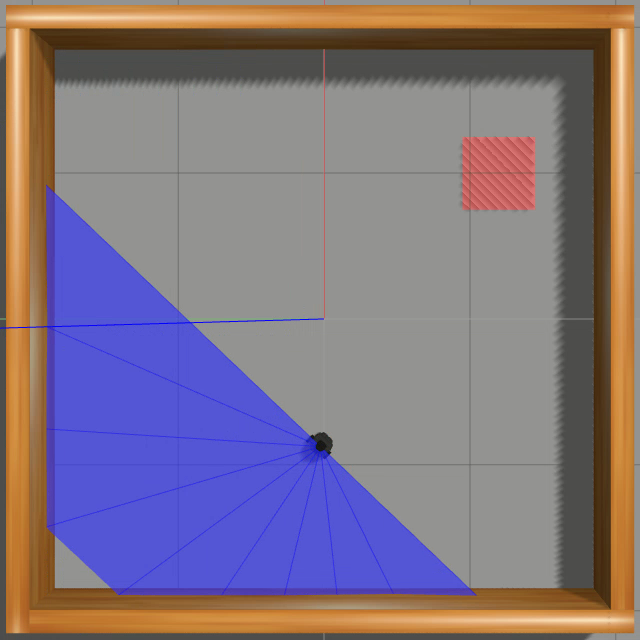
\includegraphics[width=\textwidth]{imagens/simulated_envs/sim_env1_ddpg/1.png}
        \end{subfigure}
        \hfill
        \begin{subfigure}[b]{0.24\textwidth}
            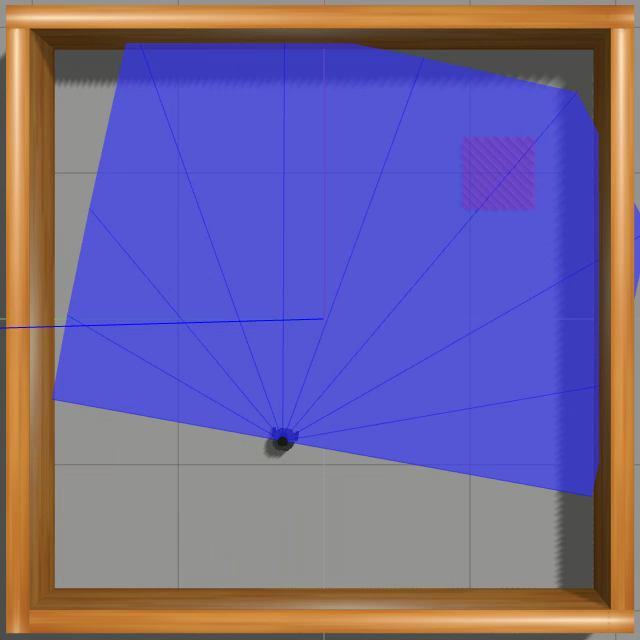
\includegraphics[width=\textwidth]{imagens/simulated_envs/sim_env1_ddpg/2.png}
        \end{subfigure}
        \hfill
        \begin{subfigure}[b]{0.24\textwidth}
            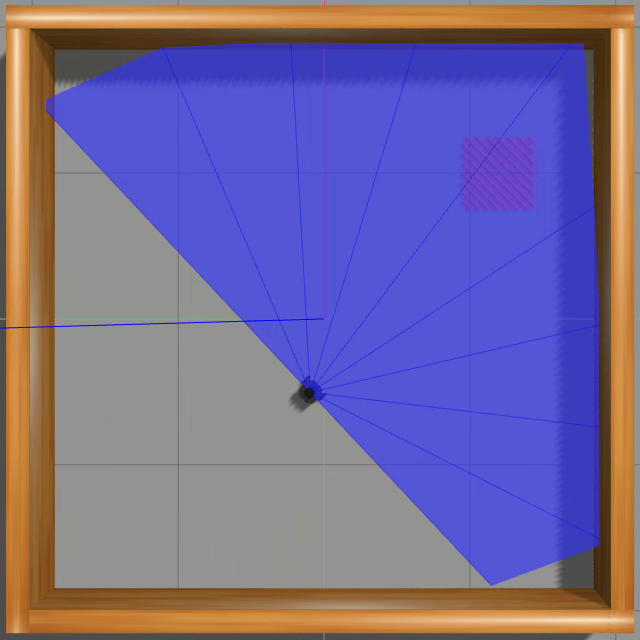
\includegraphics[width=\textwidth]{imagens/simulated_envs/sim_env1_ddpg/3.png}
        \end{subfigure}
        \hfill
        \begin{subfigure}[b]{0.24\textwidth}
            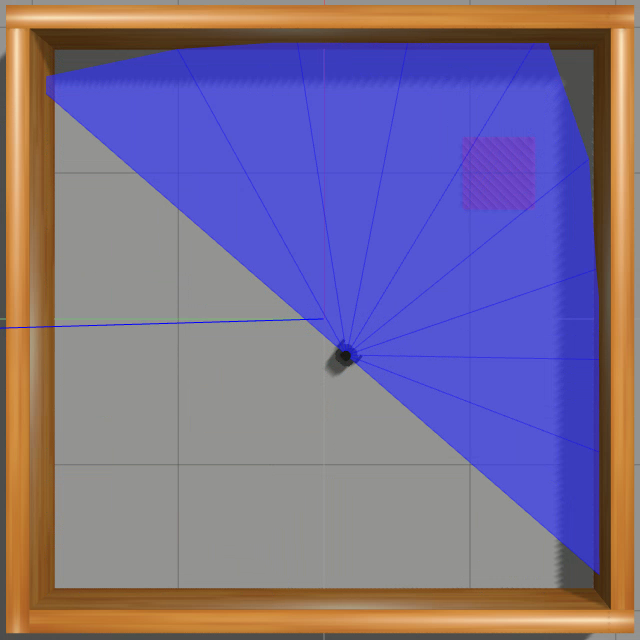
\includegraphics[width=\textwidth]{imagens/simulated_envs/sim_env1_ddpg/4.png}
        \end{subfigure}
        
        \begin{subfigure}[b]{0.24\textwidth}
            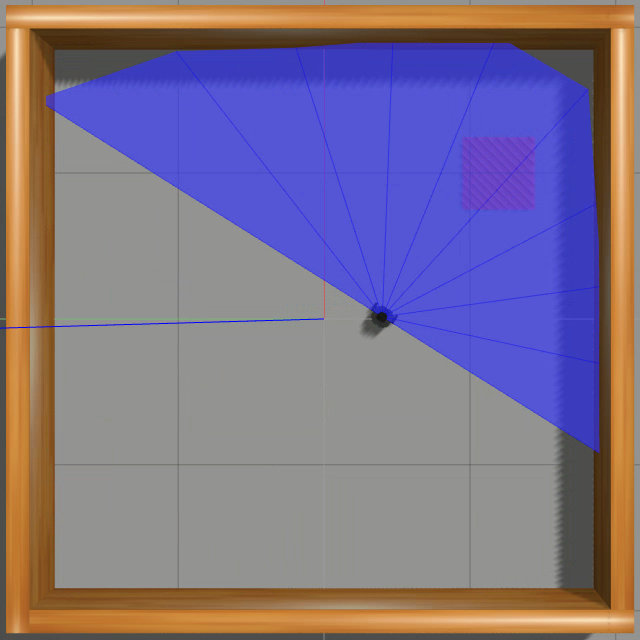
\includegraphics[width=\textwidth]{imagens/simulated_envs/sim_env1_ddpg/5.png}
        \end{subfigure}
        \hfill
        \begin{subfigure}[b]{0.24\textwidth}
            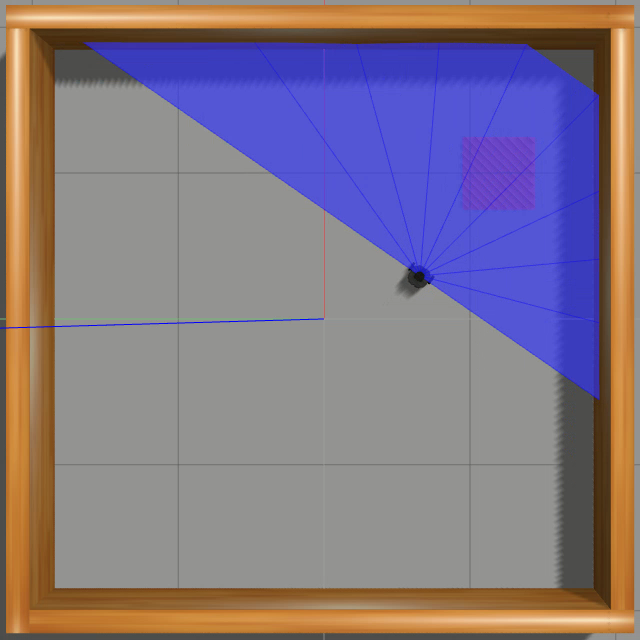
\includegraphics[width=\textwidth]{imagens/simulated_envs/sim_env1_ddpg/6.png}
        \end{subfigure}
        \hfill
        \begin{subfigure}[b]{0.24\textwidth}
            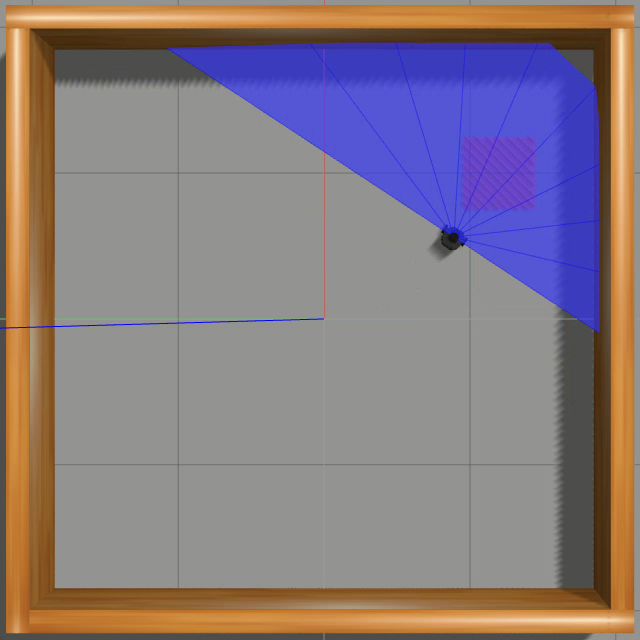
\includegraphics[width=\textwidth]{imagens/simulated_envs/sim_env1_ddpg/7.png}
        \end{subfigure}
        \hfill
        \begin{subfigure}[b]{0.24\textwidth}
            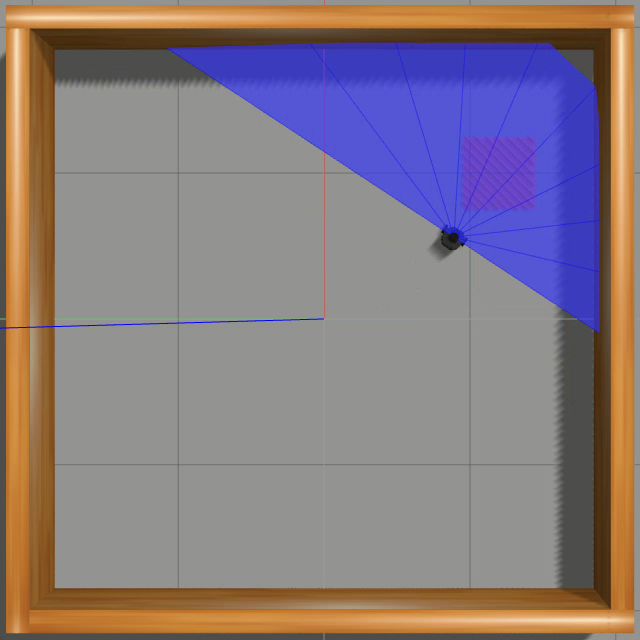
\includegraphics[width=\textwidth]{imagens/simulated_envs/sim_env1_ddpg/7.png}
        \end{subfigure}
        \caption{Rede DDPG}
        \label{subfig:simulated_env1_ddpg}
    \end{subfigure}
     %add desired spacing between images, e. g. ~, \quad, \qquad, \hfill etc. 
      %(or a blank line to force the subfigure onto a new line)
      
    \begin{subfigure}[b]{0.60\textwidth}
        \begin{subfigure}[b]{0.24\textwidth}
            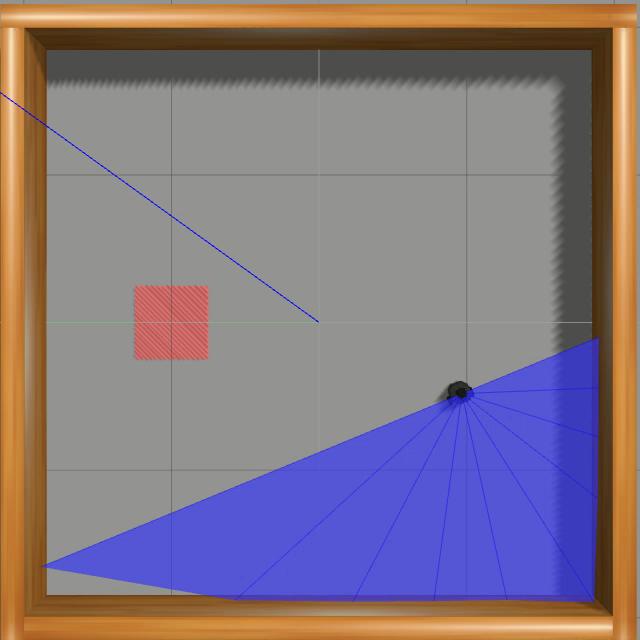
\includegraphics[width=\textwidth]{imagens/simulated_envs/sim_env1_sac/1.png}
        \end{subfigure}
        \hfill
        \begin{subfigure}[b]{0.24\textwidth}
            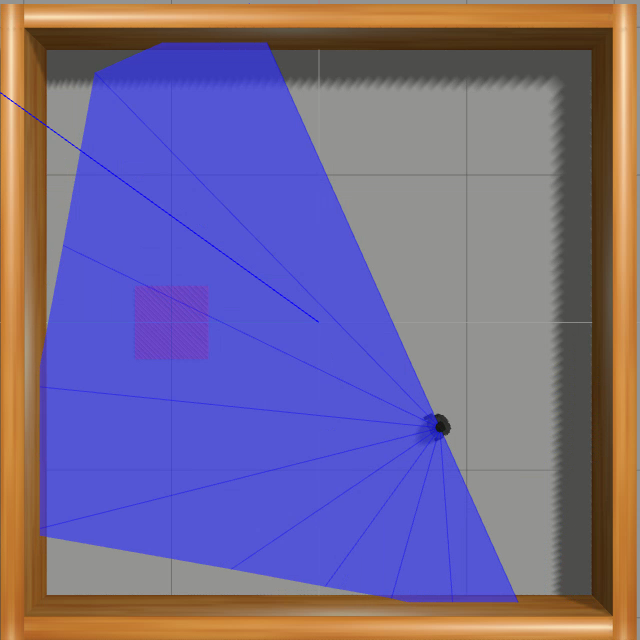
\includegraphics[width=\textwidth]{imagens/simulated_envs/sim_env1_sac/2.png}
        \end{subfigure}
        \hfill
        \begin{subfigure}[b]{0.24\textwidth}
            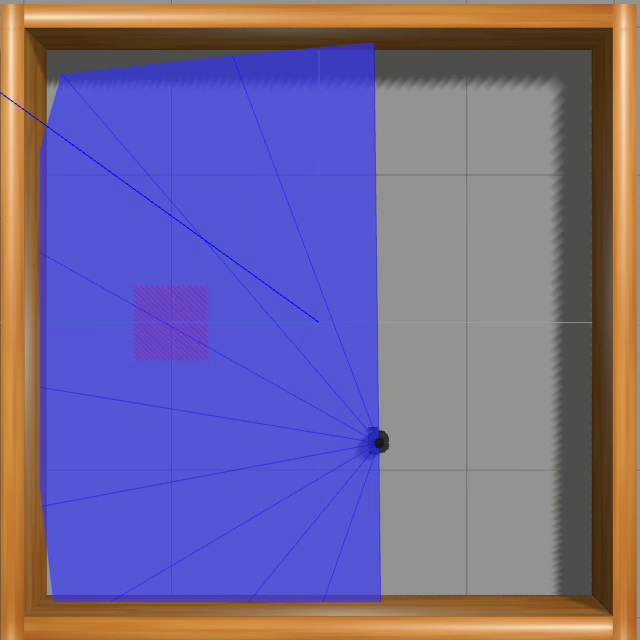
\includegraphics[width=\textwidth]{imagens/simulated_envs/sim_env1_sac/3.png}
        \end{subfigure}
        \hfill
        \begin{subfigure}[b]{0.24\textwidth}
            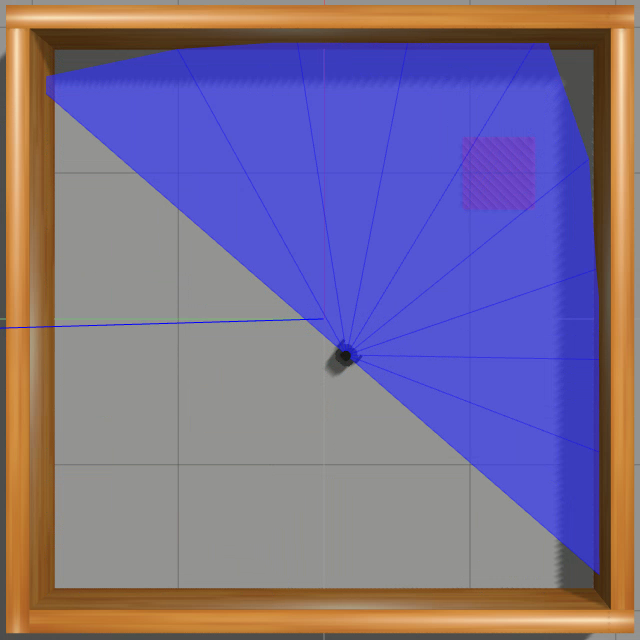
\includegraphics[width=\textwidth]{imagens/simulated_envs/sim_env1_ddpg/4.png}
        \end{subfigure}
        
        \begin{subfigure}[b]{0.24\textwidth}
            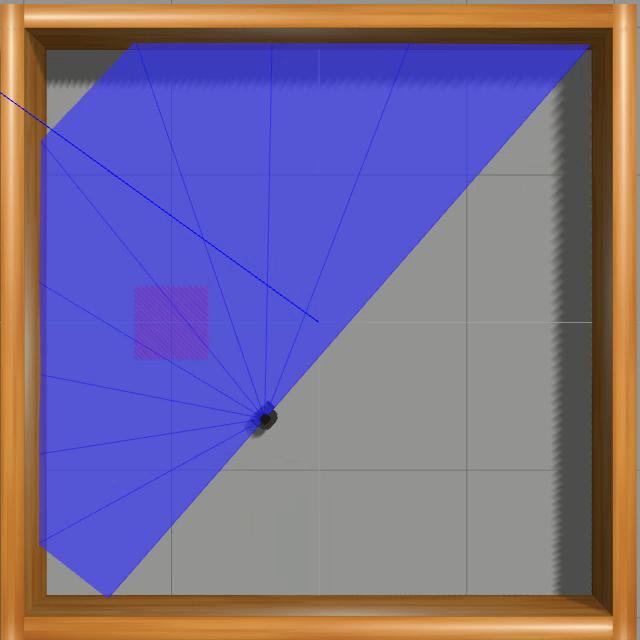
\includegraphics[width=\textwidth]{imagens/simulated_envs/sim_env1_sac/5.png}
        \end{subfigure}
        \hfill
        \begin{subfigure}[b]{0.24\textwidth}
            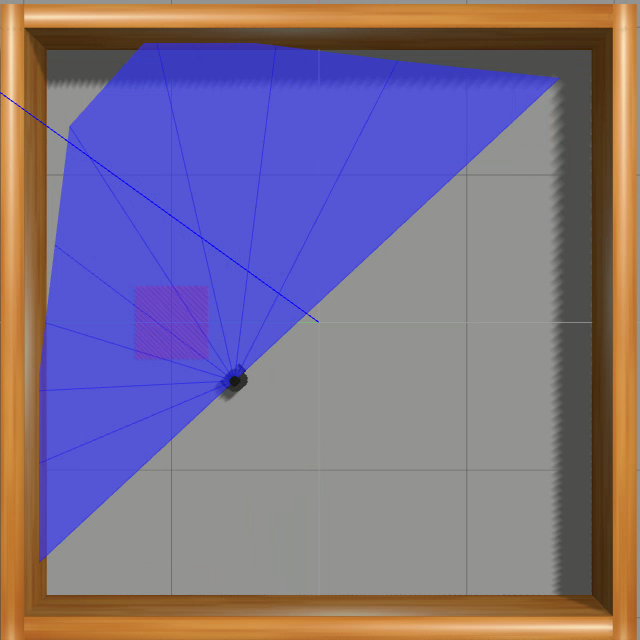
\includegraphics[width=\textwidth]{imagens/simulated_envs/sim_env1_sac/6.png}
        \end{subfigure}
        \hfill
        \begin{subfigure}[b]{0.24\textwidth}
            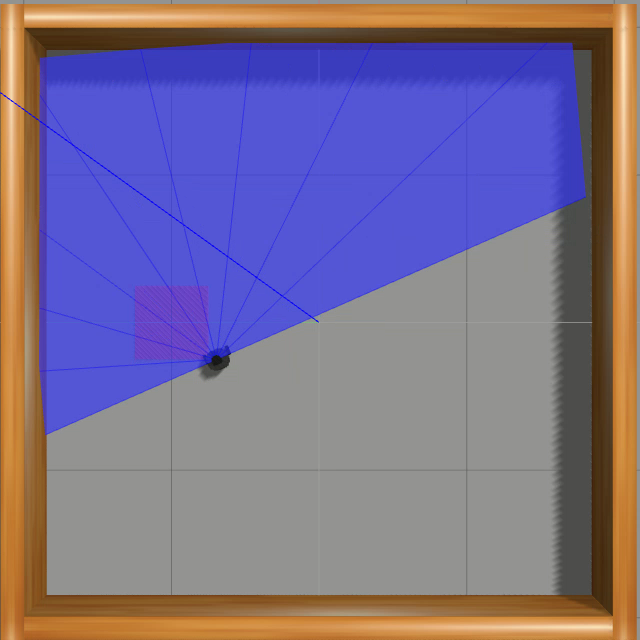
\includegraphics[width=\textwidth]{imagens/simulated_envs/sim_env1_sac/7.png}
        \end{subfigure}
        \hfill
        \begin{subfigure}[b]{0.24\textwidth}
            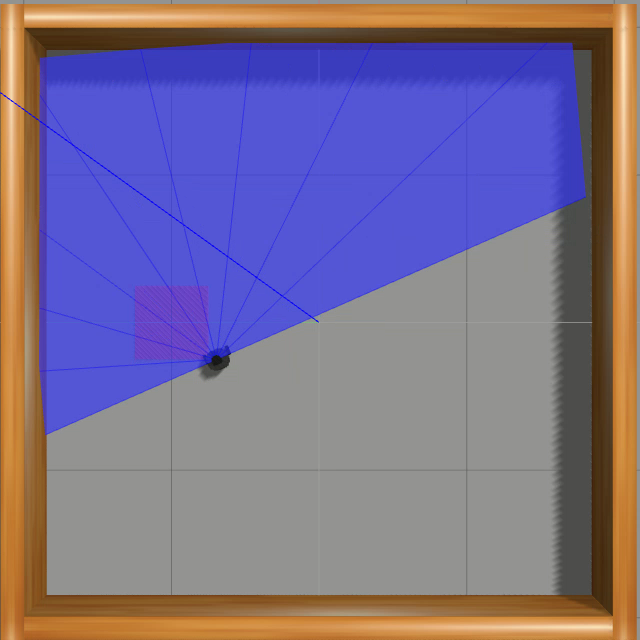
\includegraphics[width=\textwidth]{imagens/simulated_envs/sim_env1_sac/7.png}
        \end{subfigure}
        \caption{Rede SAC}
        \label{subfig:simulated_env1_sac}
    \end{subfigure}
    \label{fig:sim_env1}
    \end{center}
\small{Fonte: Autor}
\end{figure}

Os resultados do treinamento da função de recompensa do primeiro ambiente, para ambas redes, são mostrados na Figura \ref{fig:stage_1}. Nos primeiros episódios de treinamento das redes é notada uma recompensa negativa.
Isso acontece pois o algoritmo começou e ainda está em aprendizado.
Essa recompensa por episódio significa que o robô está tentando maximizar a recompensa da tarefa.
Na rede DDPG, na Figura \ref{subfig:ddpg_stage_1}, é possível ver que ela levou mais episódio para adquirir a mesma recompensa por episódio em comparação com a rede SAC, na Figura \ref{subfig:sac_stage_1}, para o mesmo episódio de treinamento.

\vspace{0.25cm}
\begin{figure}[H]
\caption{Recompensas do primeiro ambiente simulado}
    \begin{center}
    \begin{subfigure}[b]{0.48\textwidth}
        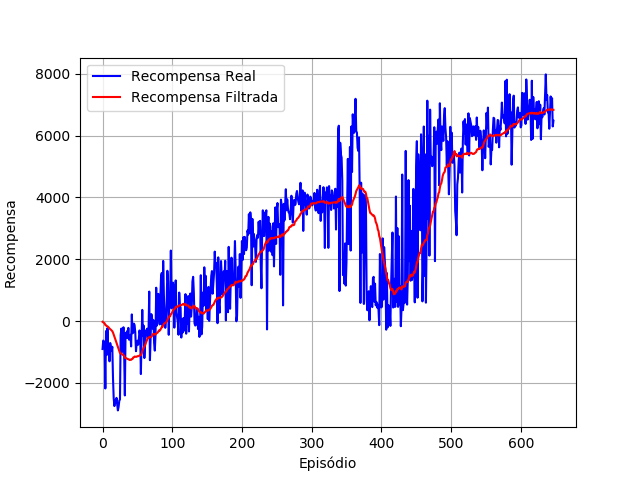
\includegraphics[width=\textwidth]{imagens/simulated_envs/ddpg_stage_1.png}
        \caption{Rede DDPG}
        \label{subfig:ddpg_stage_1}
    \end{subfigure}
    ~
    \begin{subfigure}[b]{0.48\textwidth}
        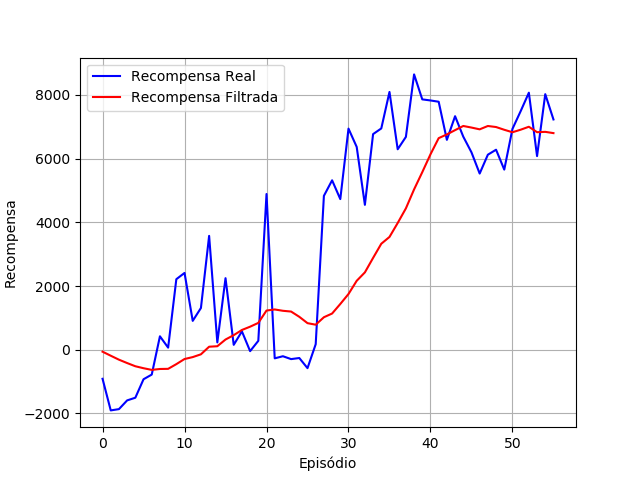
\includegraphics[width=\textwidth]{imagens/simulated_envs/sac_stage_1.png}
        \caption{Rede SAC}
        \label{subfig:sac_stage_1}
    \end{subfigure}
    \end{center}
    \label{fig:stage_1}
\small{Fonte: Autor}
\end{figure}

Na Figura \ref{fig:stage_1} o eixo $x$ representa os episódios passados na simulação, um episódio é definido quando o robô móvel chega até o alvo no mapa ou colide com algum obstáculo.
O eixo $y$, na Figura \ref{fig:stage_1}, representa o valor total da recompensa que o agente recebeu no episódio.
A recompensa, com a cor azul, tem uma grande variância. Foi decidido usar um filtro de médio móvel para melhorar a visualização dos resultados obtidos.

Depois do robô móvel ter sido treinado no primeiro ambiente, o experimento foi feito no segundo ambiente de simulação.
É mostrado na Figura \ref{fig:sim_env2} uma sequência de ações feitas pelo Turtlebot de uma posição inicial até que ele possa chegar ao alvo depois dos episódios de treinamento.

\vspace{0.25cm}
\begin{figure}[H]
\caption{Imagens sequência no segundo ambiente simulado do experimento}
    \begin{center}
    \begin{subfigure}[b]{0.60\textwidth}
        \begin{subfigure}[b]{0.24\textwidth}
            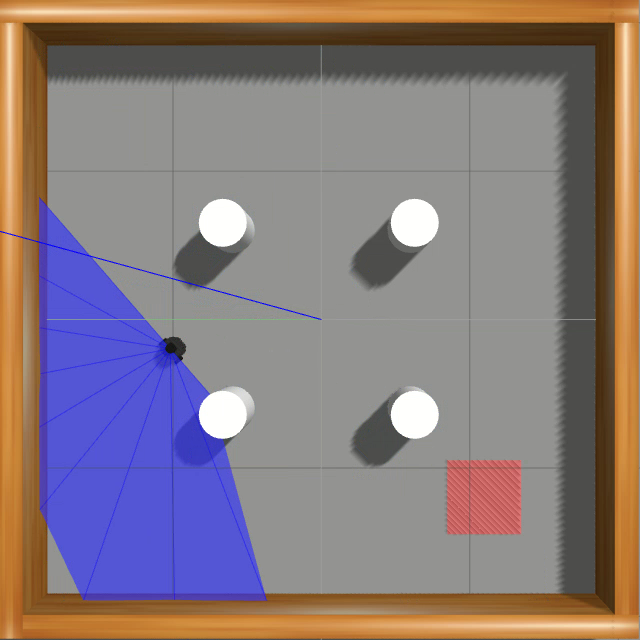
\includegraphics[width=\textwidth]{imagens/simulated_envs/sim_env2_ddpg/1.png}
        \end{subfigure}
        \hfill
        \begin{subfigure}[b]{0.24\textwidth}
            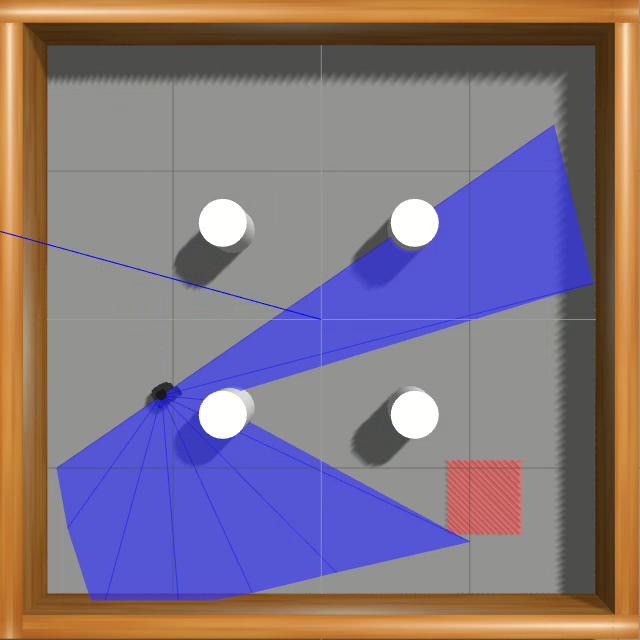
\includegraphics[width=\textwidth]{imagens/simulated_envs/sim_env2_ddpg/2.png}
        \end{subfigure}
        \hfill
        \begin{subfigure}[b]{0.24\textwidth}
            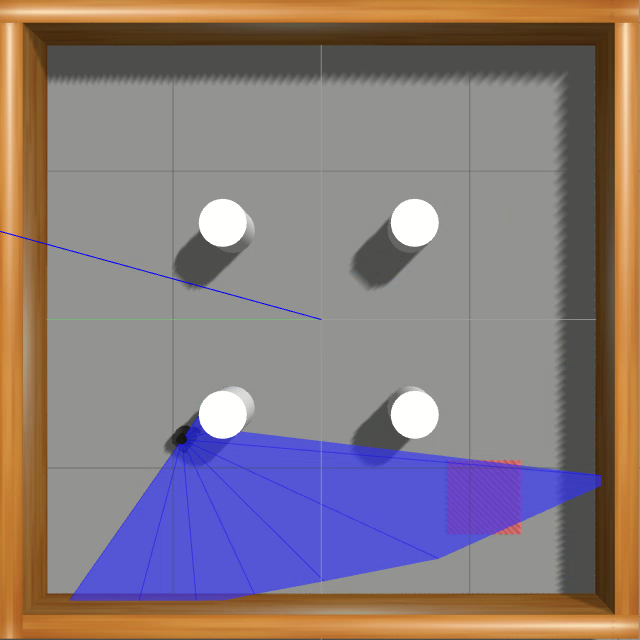
\includegraphics[width=\textwidth]{imagens/simulated_envs/sim_env2_ddpg/3.png}
        \end{subfigure}
        \hfill
        \begin{subfigure}[b]{0.24\textwidth}
            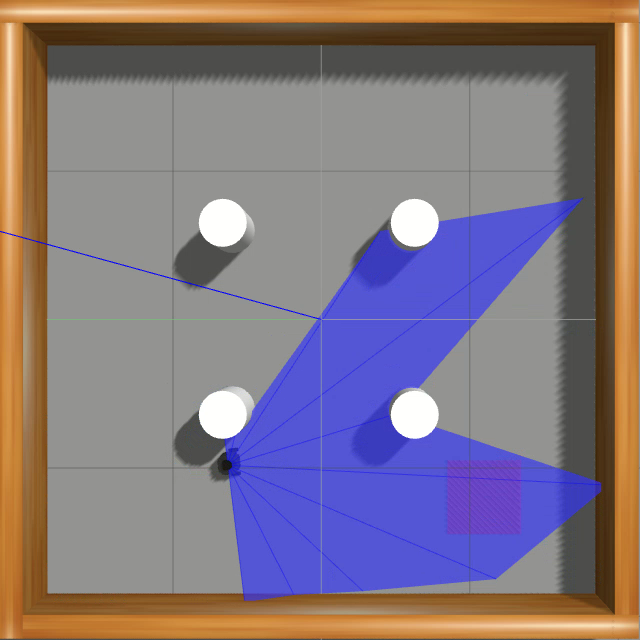
\includegraphics[width=\textwidth]{imagens/simulated_envs/sim_env2_ddpg/4.png}
        \end{subfigure}
        
        \begin{subfigure}[b]{0.24\textwidth}
            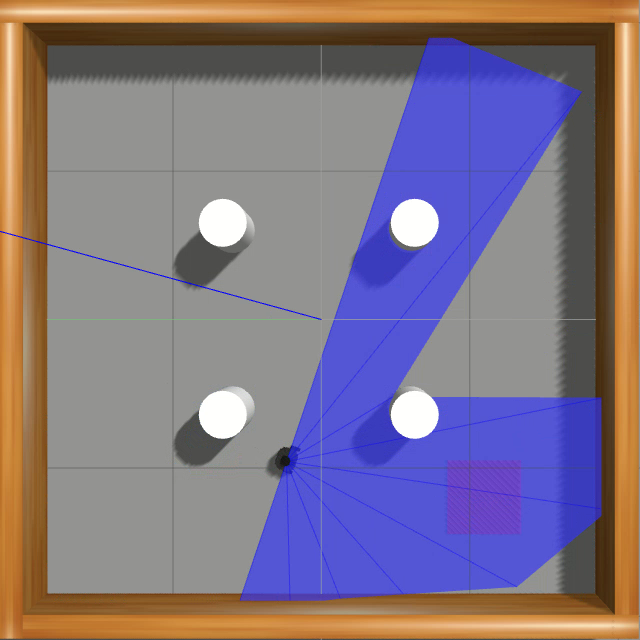
\includegraphics[width=\textwidth]{imagens/simulated_envs/sim_env2_ddpg/5.png}
        \end{subfigure}
        \hfill
        \begin{subfigure}[b]{0.24\textwidth}
            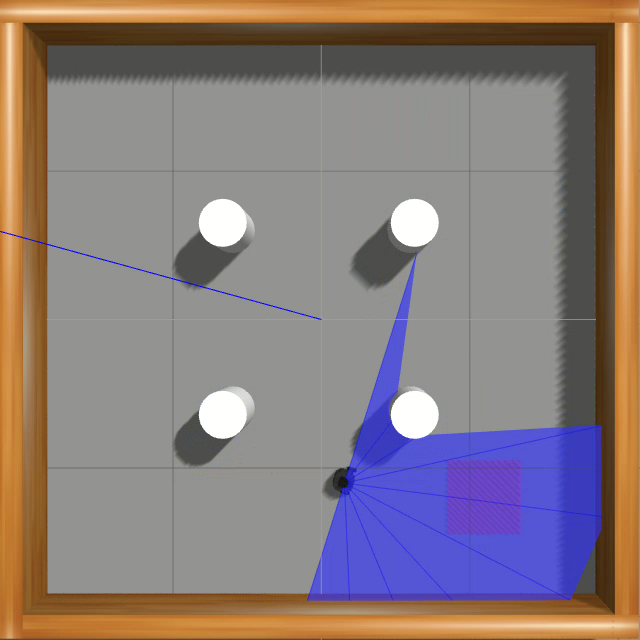
\includegraphics[width=\textwidth]{imagens/simulated_envs/sim_env2_ddpg/6.png}
        \end{subfigure}
        \hfill
        \begin{subfigure}[b]{0.24\textwidth}
            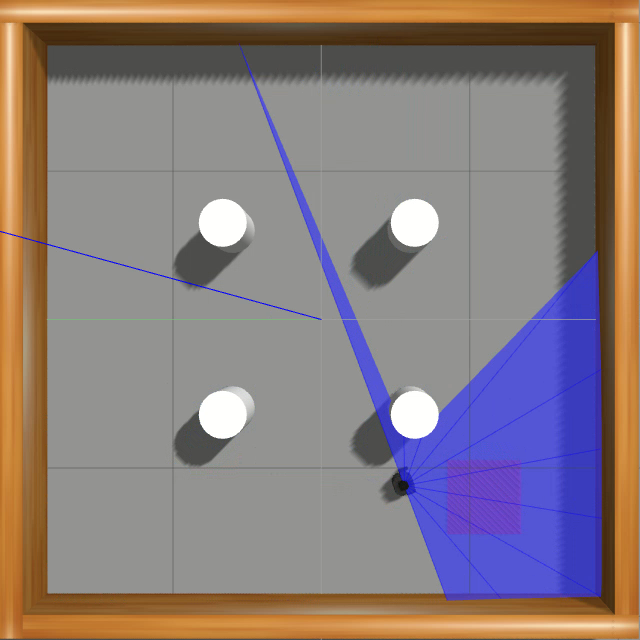
\includegraphics[width=\textwidth]{imagens/simulated_envs/sim_env2_ddpg/7.png}
        \end{subfigure}
        \hfill
        \begin{subfigure}[b]{0.24\textwidth}
            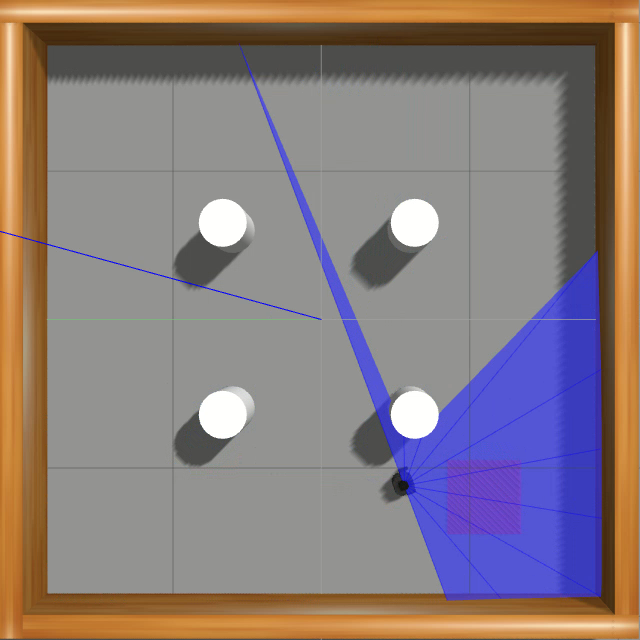
\includegraphics[width=\textwidth]{imagens/simulated_envs/sim_env2_ddpg/7.png}
        \end{subfigure}
        \caption{Rede DDPG}
        \label{subfig:simulated_env2_ddpg}
    \end{subfigure}
     %add desired spacing between images, e. g. ~, \quad, \qquad, \hfill etc. 
      %(or a blank line to force the subfigure onto a new line)
      
    \begin{subfigure}[b]{0.60\textwidth}
        \begin{subfigure}[b]{0.24\textwidth}
            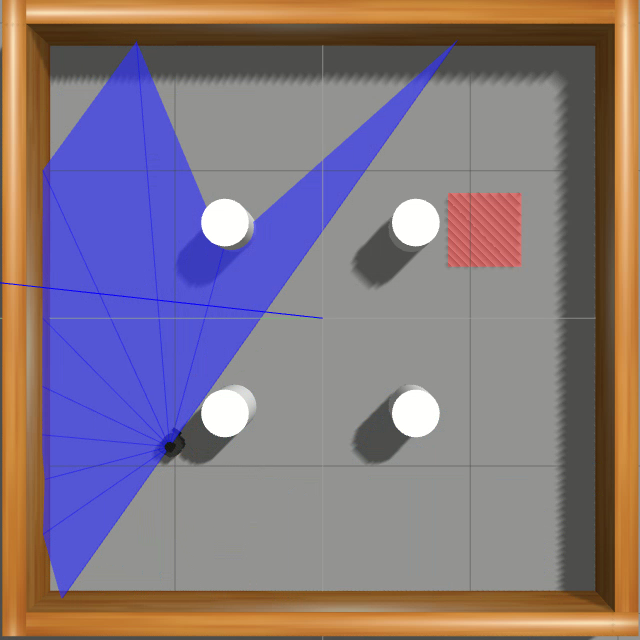
\includegraphics[width=\textwidth]{imagens/simulated_envs/sim_env2_sac/1.png}
        \end{subfigure}
        \hfill
        \begin{subfigure}[b]{0.24\textwidth}
            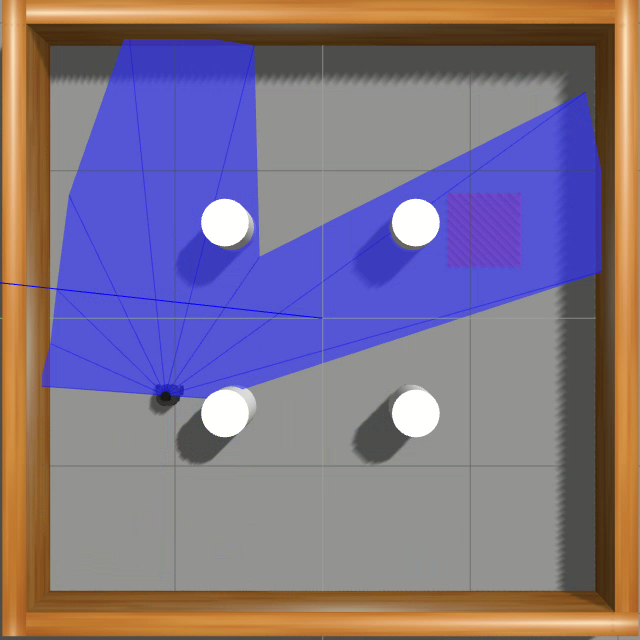
\includegraphics[width=\textwidth]{imagens/simulated_envs/sim_env2_sac/2.png}
        \end{subfigure}
        \hfill
        \begin{subfigure}[b]{0.24\textwidth}
            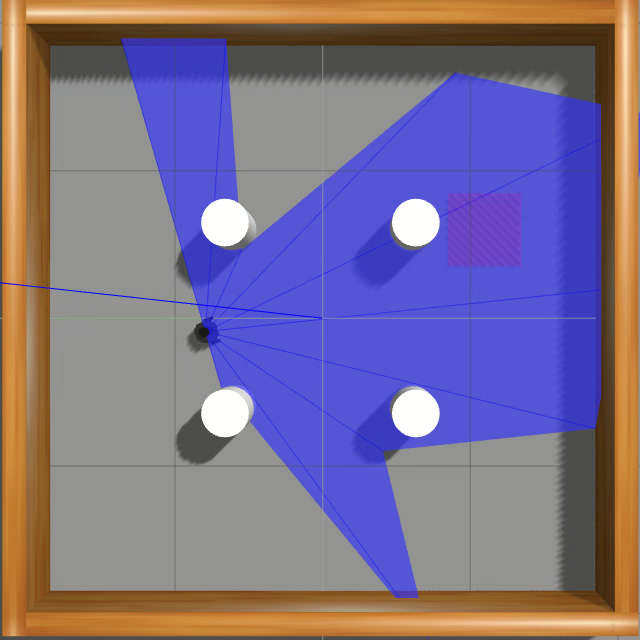
\includegraphics[width=\textwidth]{imagens/simulated_envs/sim_env2_sac/3.png}
        \end{subfigure}
        \hfill
        \begin{subfigure}[b]{0.24\textwidth}
            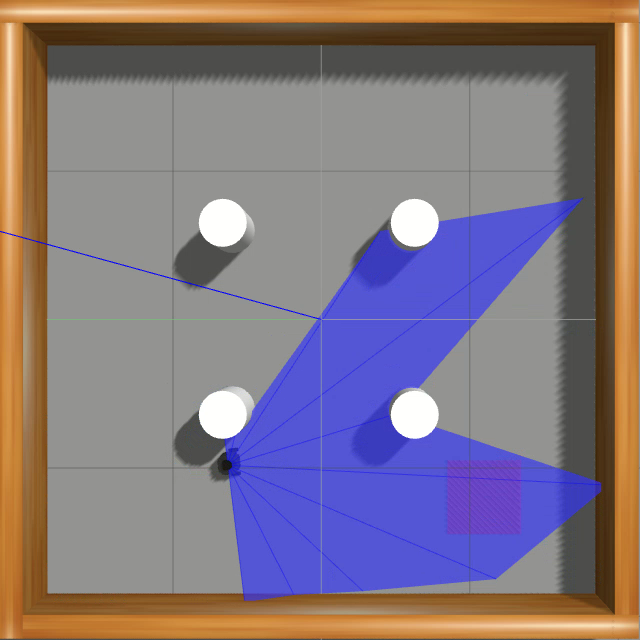
\includegraphics[width=\textwidth]{imagens/simulated_envs/sim_env2_ddpg/4.png}
        \end{subfigure}
        
        \begin{subfigure}[b]{0.24\textwidth}
            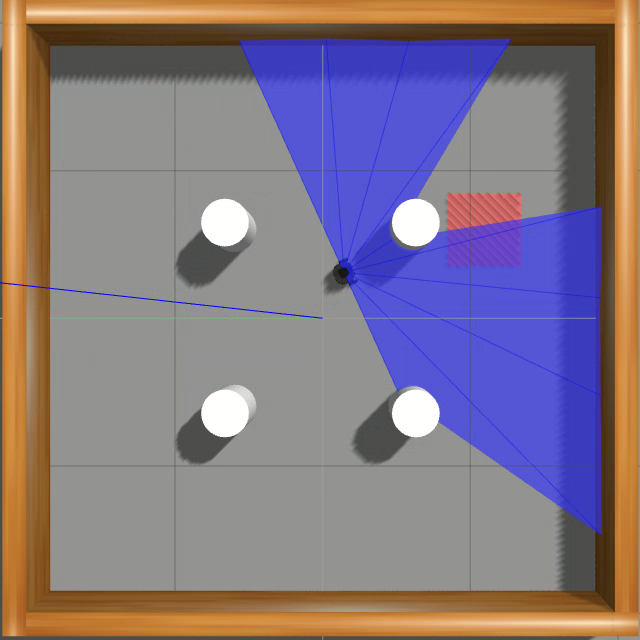
\includegraphics[width=\textwidth]{imagens/simulated_envs/sim_env2_sac/5.png}
        \end{subfigure}
        \hfill
        \begin{subfigure}[b]{0.24\textwidth}
            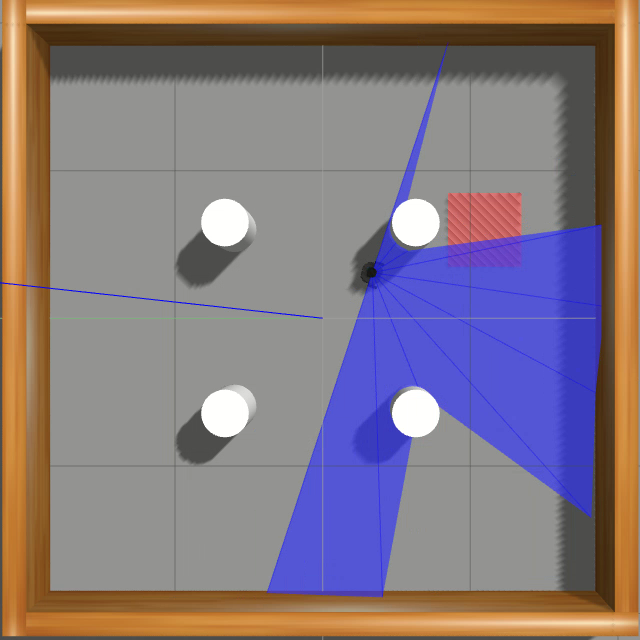
\includegraphics[width=\textwidth]{imagens/simulated_envs/sim_env2_sac/6.png}
        \end{subfigure}
        \hfill
        \begin{subfigure}[b]{0.24\textwidth}
            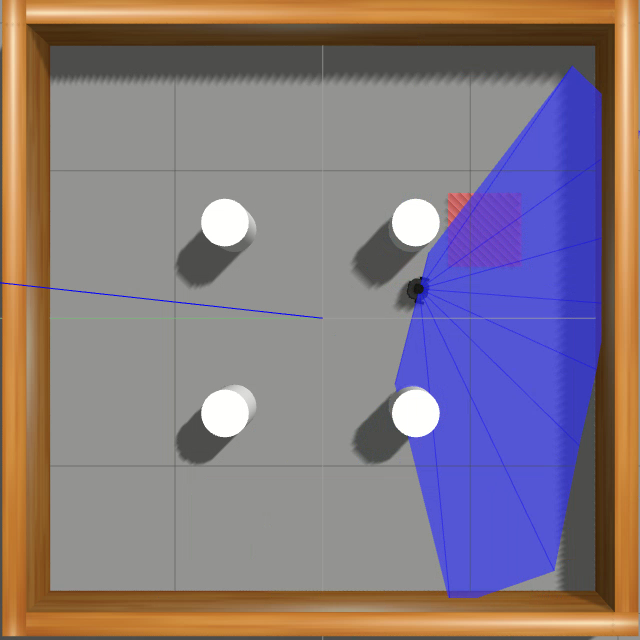
\includegraphics[width=\textwidth]{imagens/simulated_envs/sim_env2_sac/7.png}
        \end{subfigure}
        \hfill
        \begin{subfigure}[b]{0.24\textwidth}
            \includegraphics[width=\textwidth]{imagens/simulated_envs/sim_env2_sac/7.png}
        \end{subfigure}
        \caption{Rede SAC}
        \label{subfig:simulated_env2_sac}
    \end{subfigure}
    \label{fig:sim_env2}
    \end{center}
\small{Fonte: Autor}
\end{figure}

Os resultados da função de recompensa para o processo de treinamento do segundo ambiente de simulação são mostrados na Figura \ref{fig:stage_2}. 
Comparando esses resultados com último ambiente de simulação, é possível observar que é preciso mais episódios para que então o robô possa apresentar melhores resultados.
É notado que com um ambiente mais complexo, existe a possibilidade que um agente possa tomar um tempo mais longo para chegar a ter um bom desempenho.
E quando é posto em comparação a rede DDPG e SAC da Figura \ref{subfig:ddpg_stage_2} e Figura \ref{subfig:sac_stage_2}, respectivamente para o segundo ambiente de simulação, é possível ver que a rede SAC levou um número menor de episódios para obter a mesma recompensa por episódio da rede DDPG. 

\vspace{0.25cm}
\begin{figure}[H]
\caption{Recompensas do segundo ambiente simulado}
    \begin{center}
    \begin{subfigure}[b]{0.48\textwidth}
        \includegraphics[width=\textwidth]{imagens/simulated_envs/ddpg_stage_2.png}
        \caption{Rede DDPG}
        \label{subfig:ddpg_stage_2}
    \end{subfigure}
    ~
    \begin{subfigure}[b]{0.48\textwidth}
        \includegraphics[width=\textwidth]{imagens/simulated_envs/sac_stage_2.png}
        \caption{Rede SAC}
        \label{subfig:sac_stage_2}
    \end{subfigure}
    \end{center}
    \label{fig:stage_2}
\small{Fonte: Autor}
\end{figure}

Para o teste final e sequência de ações feitas pelo Turtlebot para chegar até o alvo depois do processo de treinamento foi usado o terceiro ambiente simulado.
Uma sequência das ações feitas pelo robô para chegar ao alvo depois dos episódios de treinamento são mostradas na Figura \ref{fig:sim_env3}.

\vspace{0.25cm}
\begin{figure}[H]
\caption{Imagens sequência no terceiro ambiente simulado do experimento}
    \begin{center}
    \begin{subfigure}[b]{0.60\textwidth}
        \begin{subfigure}[b]{0.24\textwidth}
            \includegraphics[width=\textwidth]{imagens/simulated_envs/sim_env3_ddpg/1.png}
        \end{subfigure}
        \hfill
        \begin{subfigure}[b]{0.24\textwidth}
            \includegraphics[width=\textwidth]{imagens/simulated_envs/sim_env3_ddpg/2.png}
        \end{subfigure}
        \hfill
        \begin{subfigure}[b]{0.24\textwidth}
            \includegraphics[width=\textwidth]{imagens/simulated_envs/sim_env3_ddpg/3.png}
        \end{subfigure}
        \hfill
        \begin{subfigure}[b]{0.24\textwidth}
            \includegraphics[width=\textwidth]{imagens/simulated_envs/sim_env3_ddpg/4.png}
        \end{subfigure}
        
        \begin{subfigure}[b]{0.24\textwidth}
            \includegraphics[width=\textwidth]{imagens/simulated_envs/sim_env3_ddpg/5.png}
        \end{subfigure}
        \hfill
        \begin{subfigure}[b]{0.24\textwidth}
            \includegraphics[width=\textwidth]{imagens/simulated_envs/sim_env3_ddpg/6.png}
        \end{subfigure}
        \hfill
        \begin{subfigure}[b]{0.24\textwidth}
            \includegraphics[width=\textwidth]{imagens/simulated_envs/sim_env3_ddpg/7.png}
        \end{subfigure}
        \hfill
        \begin{subfigure}[b]{0.24\textwidth}
            \includegraphics[width=\textwidth]{imagens/simulated_envs/sim_env3_ddpg/7.png}
        \end{subfigure}
        \caption{Rede DDPG}
        \label{subfig:simulated_env3_ddpg}
    \end{subfigure}
     %add desired spacing between images, e. g. ~, \quad, \qquad, \hfill etc. 
      %(or a blank line to force the subfigure onto a new line)
      
    \begin{subfigure}[b]{0.60\textwidth}
        \begin{subfigure}[b]{0.24\textwidth}
            \includegraphics[width=\textwidth]{imagens/simulated_envs/sim_env3_sac/1.png}
        \end{subfigure}
        \hfill
        \begin{subfigure}[b]{0.24\textwidth}
            \includegraphics[width=\textwidth]{imagens/simulated_envs/sim_env3_sac/2.png}
        \end{subfigure}
        \hfill
        \begin{subfigure}[b]{0.24\textwidth}
            \includegraphics[width=\textwidth]{imagens/simulated_envs/sim_env3_sac/3.png}
        \end{subfigure}
        \hfill
        \begin{subfigure}[b]{0.24\textwidth}
            \includegraphics[width=\textwidth]{imagens/simulated_envs/sim_env3_ddpg/4.png}
        \end{subfigure}
        
        \begin{subfigure}[b]{0.24\textwidth}
            \includegraphics[width=\textwidth]{imagens/simulated_envs/sim_env3_sac/5.png}
        \end{subfigure}
        \hfill
        \begin{subfigure}[b]{0.24\textwidth}
            \includegraphics[width=\textwidth]{imagens/simulated_envs/sim_env3_sac/6.png}
        \end{subfigure}
        \hfill
        \begin{subfigure}[b]{0.24\textwidth}
            \includegraphics[width=\textwidth]{imagens/simulated_envs/sim_env3_sac/7.png}
        \end{subfigure}
        \hfill
        \begin{subfigure}[b]{0.24\textwidth}
            \includegraphics[width=\textwidth]{imagens/simulated_envs/sim_env3_sac/7.png}
        \end{subfigure}
        \caption{Rede SAC}
        \label{subfig:simulated_env3_sac}
    \end{subfigure}
    \label{fig:sim_env3}
    \end{center}
\small{Fonte: Autor}
\end{figure}

Os resultados da função de recompensa do último ambiente de treinamento é mostrado na Figura \ref{fig:stage_4}. 
Neste ambiente, por causa da alta complexidade, foi necessário um numero maior de episódios de treinamento.
Se comparado com as funções de recompensa anterior, da Figura \ref{fig:stage_1} e Figura \ref{fig:stage_4}, é possível notar uma recompensa média abaixo de dois mil para a rede DDPG da Figura \ref{subfig:ddpg_stage_4}.
Isso acontece pois para chegar ao alvo, que tem a maior recompensa possível em comparação com as outras recompensas, é necessário que o agente possa executar ações que geram menos pontos, contudo a rede DDPG ainda consegue chegar até o alvo. 
Já se for analisada a Figura \ref{subfig:sac_stage_4}, é visto que só nos primeiros episódios iniciais que ela apresenta um recompensa por episódio menor que dois mil, sem falar no menor tempo de treinos para ela superar a rede DDPG mesmo em relação ao treinamento do segundo ambiente que é mais simples que o terceiro ambiente de simulado.
Apesar disso, foi notado simulando o robô treinado algumas ações que causam o agente a colidir.
Muita dessas colisões foram devidas ao obstáculo dinâmico em movimento perto do alvo.
Isso resultou no agente fazer a decisão de que Turtlebot simulado poderia colidir ou tentar evitar o obstaculo móvel.
O comportamento ocorrido pode ter sido causado por causa do sistema de recompensa criado.
Em ordem de resolver essas ações, provavelmente, seria necessário criar uma função de recompensa que pudesse ignorar o erro para as redes treinadas.

\vspace{0.25cm} 
\begin{figure}[H]
\caption{Recompensas do terceiro ambiente simulado}
    \begin{center}
    \begin{subfigure}[b]{0.48\textwidth}
        \includegraphics[width=\textwidth]{imagens/simulated_envs/ddpg_stage_4.png}
        \caption{Rede DDPG}
        \label{subfig:ddpg_stage_4}
    \end{subfigure}
    ~
    \begin{subfigure}[b]{0.48\textwidth}
        \includegraphics[width=\textwidth]{imagens/simulated_envs/sac_stage_4.png}
        \caption{Rede SAC}
        \label{subfig:sac_stage_4}
    \end{subfigure}
    \end{center}
    \label{fig:stage_4}
\small{Fonte: Autor}
\end{figure}

%% escrever algo aqui. tipo "como notado nas recompensas da figura tal, figura tal e figural tal, a rede sac apresentou resultados melhores que a rede ddpg"
%%
%%
%%
%%
%%

\section{Experimentos com Turtlebot em Ambiente Real}

Depois do treinamento e validação de cada ambiente de simulação, foram utilizados dois ambientes reais, apresentados na Figura \ref{fig:real_environments}, para testar a rede DDPG e SAC no mundo real.
Com o alvo definido no primeiro no primeiro ambiente real, foram executadas a rede DDPG e SAC no Turtlebot3 versão Burger.
Nos gráficos, mostrados na Figura \ref{fig:real_env1}, é possível ver a trajetória feita pela rede DDPG e SAC  para chegar até o alvo.
O robô começa no ponto $(0,0)$ e faz uma trajetória para conseguir ir ao alvo.
É possível ver que ambas as redes, DDPG e SAC, conseguiram chegar ao alvo definido em um ambiente real.
A Figura \ref{fig:real_env1_frames} mostra por quadros de imagem a trajetória feita pelo robô para completar a tarefa.

\vspace{0.25cm} 
\begin{figure}[H]
\caption{Trajetória do Turtlebot3 no primeiro ambiente real}
    \begin{center}
    \begin{subfigure}[b]{0.48\textwidth}
        \includegraphics[width=\textwidth]{imagens/real_envs/real_env1_ddpg/graph.png}
        \caption{Rede DDPG}
        \label{subfig:ddpg_real_env1}
    \end{subfigure}
    ~
    \begin{subfigure}[b]{0.48\textwidth}
        \includegraphics[width=\textwidth]{imagens/real_envs/real_env1_sac/graph.png}
        \caption{Rede SAC}
        \label{subfig:sac_real_env1}
    \end{subfigure}
    \end{center}
    \label{fig:real_env1}
\small{Fonte: Autor}
\end{figure}

% ibagens
\vspace{0.25cm}
\begin{figure}[H]
\caption{Imagens sequência do experimento no Turtlebot3 no primeiro ambiente real}
    \begin{center}
    \begin{subfigure}[b]{0.60\textwidth}
        \begin{subfigure}[b]{0.24\textwidth}
            \includegraphics[width=\textwidth]{imagens/real_envs/real_env1_ddpg/1.png}
        \end{subfigure}
        \hfill
        \begin{subfigure}[b]{0.24\textwidth}
            \includegraphics[width=\textwidth]{imagens/real_envs/real_env1_ddpg/2.png}
        \end{subfigure}
        \hfill
        \begin{subfigure}[b]{0.24\textwidth}
            \includegraphics[width=\textwidth]{imagens/real_envs/real_env1_ddpg/3.png}
        \end{subfigure}
        \hfill
        \begin{subfigure}[b]{0.24\textwidth}
            \includegraphics[width=\textwidth]{imagens/real_envs/real_env1_ddpg/4.png}
        \end{subfigure}
        
        \begin{subfigure}[b]{0.24\textwidth}
            \includegraphics[width=\textwidth]{imagens/real_envs/real_env1_ddpg/5.png}
        \end{subfigure}
        \hfill
        \begin{subfigure}[b]{0.24\textwidth}
            \includegraphics[width=\textwidth]{imagens/real_envs/real_env1_ddpg/6.png}
        \end{subfigure}
        \hfill
        \begin{subfigure}[b]{0.24\textwidth}
            \includegraphics[width=\textwidth]{imagens/real_envs/real_env1_ddpg/7.png}
        \end{subfigure}
        \hfill
        \begin{subfigure}[b]{0.24\textwidth}
            \includegraphics[width=\textwidth]{imagens/real_envs/real_env1_ddpg/7.png}
        \end{subfigure}
        \caption{Rede DDPG}
        \label{subfig:real_env1_ddpg}
    \end{subfigure}
     %add desired spacing between images, e. g. ~, \quad, \qquad, \hfill etc. 
      %(or a blank line to force the subfigure onto a new line)
      
    \begin{subfigure}[b]{0.60\textwidth}
        \begin{subfigure}[b]{0.24\textwidth}
            \includegraphics[width=\textwidth]{imagens/real_envs/real_env1_sac/1.png}
        \end{subfigure}
        \hfill
        \begin{subfigure}[b]{0.24\textwidth}
            \includegraphics[width=\textwidth]{imagens/real_envs/real_env1_sac/2.png}
        \end{subfigure}
        \hfill
        \begin{subfigure}[b]{0.24\textwidth}
            \includegraphics[width=\textwidth]{imagens/real_envs/real_env1_sac/3.png}
        \end{subfigure}
        \hfill
        \begin{subfigure}[b]{0.24\textwidth}
            \includegraphics[width=\textwidth]{imagens/real_envs/real_env1_ddpg/4.png}
        \end{subfigure}
        
        \begin{subfigure}[b]{0.24\textwidth}
            \includegraphics[width=\textwidth]{imagens/real_envs/real_env1_sac/5.png}
        \end{subfigure}
        \hfill
        \begin{subfigure}[b]{0.24\textwidth}
            \includegraphics[width=\textwidth]{imagens/real_envs/real_env1_sac/6.png}
        \end{subfigure}
        \hfill
        \begin{subfigure}[b]{0.24\textwidth}
            \includegraphics[width=\textwidth]{imagens/real_envs/real_env1_sac/7.png}
        \end{subfigure}
        \hfill
        \begin{subfigure}[b]{0.24\textwidth}
            \includegraphics[width=\textwidth]{imagens/real_envs/real_env1_sac/7.png}
        \end{subfigure}
        \caption{Rede SAC}
        \label{subfig:real_env1_sac}
    \end{subfigure}
    \label{fig:real_env1_frames}
    \end{center}
\small{Fonte: Autor}
\end{figure}

Para o teste final das redes, foi usado o segundo ambiente real. Nos gráficos, mostrados na Figura \ref{fig:real_env2}, o robô começa no ponto $(0,0)$ e mesmo com obstáculos a rede DDPG e SAC são capazes de chegar ao alvo do ambiente.
Na Figura \ref{fig:real_env2_frames} é mostrado por quadros de imagem a trajetória feita pelo robô móvel para completar a tarefa.

\vspace{0.25cm} 
\begin{figure}[H]
\caption{Trajetória do Turtlebot3 no segundo ambiente real}
    \begin{center}
    \begin{subfigure}[b]{0.48\textwidth}
        \includegraphics[width=\textwidth]{imagens/real_envs/real_env2_ddpg/graph.png}
        \caption{Rede DDPG}
        \label{subfig:ddpg_real_env2}
    \end{subfigure}
    ~
    \begin{subfigure}[b]{0.48\textwidth}
        \includegraphics[width=\textwidth]{imagens/real_envs/real_env2_sac/graph.png}
        \caption{Rede SAC}
        \label{subfig:sac_real_env2}
    \end{subfigure}
    \end{center}
    \label{fig:real_env2}
\small{Fonte: Autor}
\end{figure}

% ibagens
\vspace{0.25cm}
\begin{figure}[H]
\caption{Imagens sequência do experimento no Turtlebot3 no segundo ambiente real}
    \begin{center}
    \begin{subfigure}[b]{0.60\textwidth}
        \begin{subfigure}[b]{0.24\textwidth}
            \includegraphics[width=\textwidth]{imagens/real_envs/real_env2_ddpg/1.png}
        \end{subfigure}
        \hfill
        \begin{subfigure}[b]{0.24\textwidth}
            \includegraphics[width=\textwidth]{imagens/real_envs/real_env2_ddpg/2.png}
        \end{subfigure}
        \hfill
        \begin{subfigure}[b]{0.24\textwidth}
            \includegraphics[width=\textwidth]{imagens/real_envs/real_env2_ddpg/3.png}
        \end{subfigure}
        \hfill
        \begin{subfigure}[b]{0.24\textwidth}
            \includegraphics[width=\textwidth]{imagens/real_envs/real_env2_ddpg/4.png}
        \end{subfigure}
        
        \begin{subfigure}[b]{0.24\textwidth}
            \includegraphics[width=\textwidth]{imagens/real_envs/real_env2_ddpg/5.png}
        \end{subfigure}
        \hfill
        \begin{subfigure}[b]{0.24\textwidth}
            \includegraphics[width=\textwidth]{imagens/real_envs/real_env2_ddpg/6.png}
        \end{subfigure}
        \hfill
        \begin{subfigure}[b]{0.24\textwidth}
            \includegraphics[width=\textwidth]{imagens/real_envs/real_env2_ddpg/7.png}
        \end{subfigure}
        \hfill
        \begin{subfigure}[b]{0.24\textwidth}
            \includegraphics[width=\textwidth]{imagens/real_envs/real_env2_ddpg/7.png}
        \end{subfigure}
        \caption{Rede DDPG}
        \label{subfig:real_env2_ddpg}
    \end{subfigure}
     %add desired spacing between images, e. g. ~, \quad, \qquad, \hfill etc. 
      %(or a blank line to force the subfigure onto a new line)
      
    \begin{subfigure}[b]{0.60\textwidth}
        \begin{subfigure}[b]{0.24\textwidth}
            \includegraphics[width=\textwidth]{imagens/real_envs/real_env2_sac/1.png}
        \end{subfigure}
        \hfill
        \begin{subfigure}[b]{0.24\textwidth}
            \includegraphics[width=\textwidth]{imagens/real_envs/real_env2_sac/2.png}
        \end{subfigure}
        \hfill
        \begin{subfigure}[b]{0.24\textwidth}
            \includegraphics[width=\textwidth]{imagens/real_envs/real_env2_sac/3.png}
        \end{subfigure}
        \hfill
        \begin{subfigure}[b]{0.24\textwidth}
            \includegraphics[width=\textwidth]{imagens/real_envs/real_env2_ddpg/4.png}
        \end{subfigure}
        
        \begin{subfigure}[b]{0.24\textwidth}
            \includegraphics[width=\textwidth]{imagens/real_envs/real_env2_sac/5.png}
        \end{subfigure}
        \hfill
        \begin{subfigure}[b]{0.24\textwidth}
            \includegraphics[width=\textwidth]{imagens/real_envs/real_env2_sac/6.png}
        \end{subfigure}
        \hfill
        \begin{subfigure}[b]{0.24\textwidth}
            \includegraphics[width=\textwidth]{imagens/real_envs/real_env2_sac/7.png}
        \end{subfigure}
        \hfill
        \begin{subfigure}[b]{0.24\textwidth}
            \includegraphics[width=\textwidth]{imagens/real_envs/real_env2_sac/7.png}
        \end{subfigure}
        \caption{Rede SAC}
        \label{subfig:real_env2_sac}
    \end{subfigure}
    \label{fig:real_env2_frames}
    \end{center}
\small{Fonte: Autor}
\end{figure}

O robô Turtlebot3 foi capaz de realizar ambas as tarefas dadas nos ambientes do mundo real.
Isso mostra o quão efetivo podem ser as redes DDPG e SAC, treinadas em ambientes de simulação, em completar tarefas complexas em ambientes físicos.
\chapter{Conclusão}

Neste trabalho uma de rede DDPG e SAC foram usadas na navegação de um robô móvel através de controle contínuo em um ambiente virtual e real.
Assim, foi mostrado que redes de aprendizado por reforço são capazes de resolver o problema de navegação robótica.
O experimento consistiu que o robô pudesse chegar a uma posição alvo em diferentes ambientes simulados e reais.
Em ordem de realizar esse objetivo a função de recompensa foi proposta.
As saídas de redes utilizadas foram a velocidade linear e angular do robô móvel.
Todas estruturas de rede criadas foram treinadas no ambiente de simulação do Gazebo antes de usar a redes em ambientes reais.

Com o resultado obtidos do treinamento no ambiente de simulação, foi analisado o desempenho dos algoritmos de agentes inteligentes na tarefa de evitar obstáculos e chegar até o seu objetivo final.
Foi notado que a rede SAC consegue em um número menor de episódios ter um desempenho superior a rede DDPG.
Nos dois ambientes reais propostos, os algoritmos foram capazes de completar a tarefa da navegação para chegar até um alvo definido no mapa, em que ambas as redes propostas no trabalho conseguiram completar com facilidade.

É possível concluir que as redes DDPG e SAC são adequadas para o desenvolvimento de aplicações que necessitam um controle contínuo na robótica. 
As técnicas de  Deep-RL podem produzir excelentes resultados se a função de recompensa proposta é bem-feita para o problema que ela quer resolver.
Foi provado que agentes inteligentes podem mover-se em um ambiente real complexo por apenas treinar em ambientes simulados sem nenhum conhecimentos prévio do cenário.
Em um futuro trabalho, é planejado fazer a utilização de redes Deep-RL para o controle de múltiplos para jogarem futebol.
%%========================================================================

\setlength{\baselineskip}{\baselineskip}

%%=============================================================================
%% Referências
%%=============================================================================
\begin{flushleft}
\bibliographystyle{abnt}
\bibliography{referencias/referencias}
\end{flushleft}

%IMPORTANTE: Se precisar usar alguma seção ou subseção dentro dos apêndices ou
%anexos, utilizar o comando \tocless para não adicionar no Sumário
%Exemplos: 
% \tocless\section{Histórico}
%%=============================================================================
%% Apêndices
%%=============================================================================
\appendix





%IMPORTANTE: Se precisar usar alguma seção ou subseção dentro dos apêndices ou
%anexos, utilizar o comando \tocless para não adicionar no Sumário
%Exemplos: 
% \tocless\section{Histórico}
% \tocless\subsection{Detalhes}
\tocless\section{teste}
%Este é um teste de seção dentro do apêndice


%
\chapter{Título do apêndice Ex}
Esta é o apêndice B



%%=============================================================================
%% Anexos
%%=============================================================================
\annex
\chapter{Título do Anexo}
Este é o anexo A



\end{document}
